\documentclass[12pt]{article}
\usepackage{amsmath}
\usepackage{csquotes} % for bibliography
\usepackage[english]{babel}
\usepackage{xcolor}
\usepackage{dcolumn}
\usepackage{graphicx} % Required for inserting images
\usepackage{multirow} %for nicer tables
\usepackage{subcaption} % subfigures
\usepackage{lscape} %to fit the tables on the page
\graphicspath{{Images/}}
\usepackage[a4paper,top=2cm,bottom=2cm,left=2cm,right=2cm]{geometry}
\setlength\parindent{0pt}
\usepackage{setspace}
\doublespacing

\usepackage{hyperref}
\hypersetup{
    colorlinks=true,
    linkcolor=black,
    filecolor=black,      
    urlcolor=blue, % for \href in data appendicies
    citecolor=black,
}
\usepackage[
    backend=biber, 
    citestyle=authoryear-comp, 
    bibstyle=authoryear, 
    url=false, 
    sorting=nyt, % order of bibliography sorted by name, year title
    hyperref=true, 
    maxcitenames=2, % use et al if more than 2
    isbn=false, 
    doi=false,  % suppress from bibliorgraphy
    giveninits=true, % initials for first names
    uniquename=false, 
    date=year % no month in bibliography
]{biblatex}
\addbibresource{references-manual.bib}
\addbibresource{zotero.bib}
\usepackage{booktabs}
\renewbibmacro{in:}{} % don't have "In: " before journal name
\renewcommand*{\nameyeardelim}{\addcomma\space}
\DeclareFieldFormat{pages}{#1}
\DeclareNameAlias{default}{family-given}
\DeclareNameAlias{sortname}{family-given}
\renewcommand{\labelnamepunct}{\addcomma\addspace} % comma separators in bibliography
\renewcommand{\newunitpunct}{\addcomma\addspace} % comma separators in bibliography
\DeclareFieldFormat[article]{number}{\addspace\mkbibparens{#1}} % wrap issue number in braces
\usepackage[printonlyused]{acronym}

% make references appear in table of contents
\usepackage[nottoc]{tocbibind}
\usepackage{placeins} % \FloatBarrier

\begin{document}
    \begin{titlepage}

\begin{center}

\vspace*{1,2cm}

\huge {\bfseries Sunlight Synchronisation: Exploring the Influence of Daylight Saving Time on CO2 Emissions and Electricity Consumption in Australia’s Electricity Grid}\\[1.8cm]

\Large {Applied Econometrics Research Paper}\\[1cm]

\large {Department of Economics}\\[0.2cm]

\large {Toulouse School of Economics}\\[0.5cm]

\end{center}

\vfill

\noindent Submitted to:\\
Jean Francois Fournel, PhD\\[0.7cm]
Submitted by:\\
Davis, Koehler, Postler \& Stegmaier\\[0.7cm]
Student IDs: 
22307993, % Matt
22308759, % Alex
22307997, % simon
22308009 % David
\\
Degree Programme: M1 (Applied) Economics International Track \\[0.7cm]
Toulouse, 19.03.2024

\setcounter{page}{0}

\end{titlepage}
    \thispagestyle{empty}
    \tableofcontents
    \clearpage
    \pagenumbering{Roman}
    \thispagestyle{empty}
    \markboth{List of Abbreviations}{List of Abbreviations}
    \addcontentsline{toc}{section}{Acronyms}
    % this both defines acronyms
% (even if they are used prior to this)
% and prints the list of acronyms
\subsection*{Acronyms}

\begin{acronym}[SP-ICPMS]
    \acro{AEMO}{the Australian Energy Market Operator} % typically people say "AEMO" not "the AEMO"
    \acro{DST}{Daylight saving time} % Saving not Savings
    \acro{DiD}{Difference-in-differences}
    \acro{DDD}{Difference-in-differences-in-differences}
    \acro{NEM}{National Electricity Market} % excludes WA and NT
    \acro{QLD}{Queensland}
    \acro{NSW}{New South Wales}
    \acro{VIC}{Victoria}
    \acro{TAS}{Tasmania}
    \acro{NT}{The Northern Territory}
    \acro{WA}{Western Australia}
    \acro{SA}{South Australia}
\end{acronym}  
    \listoffigures
    \listoftables
    \newpage
    \pagenumbering{arabic}
    \setcounter{page}{1}
    
\section{Introduction}
%We propose researching the question: "". Given the recent trend in ... given then recent debates surrounding ... researching ...
\ac{DST} describes the practice of advancing clocks by one hour during the summer months of the year. For people whose daily schedule is based on clock time, this means that the sun appears to rise and set one hour earlier and they experience an additional hour of sunlight each day, as shown in Figure \ref{fig:sunrise plot}. Today approximately 70 countries have adopted \ac{DST} as a policy \parencite{prerau_book}. Since \ac{DST} was first introduced, the electricity industry has changed drastically. Solar generation is becoming more and more commonplace and inefficient compact fluorescent bulbs have been replaced with far more efficient LEDs. Today, lighting makes up only 15\% of the overall electrical load worldwide \parencite{ec_lighting}. 
Despite being widely adopted over the last century, there is only moderate evidence to support the original energy-saving motivation for \ac{DST} \parencite{prerau_book}. Most literature suggests that \ac{DST} merely shifts load from the evening to the morning, causing a negligible net reduction in electricity consumption, or even a slight increase \parencite{kellogg_daylight_2008, aries_effect_2008, guven}.
In terms of emissions (and cost reduction), shifting \textit{when} consumers consume electricity can be as impactful as reducing the volume consumed \parencite{holland_is_2008}.

We propose that \ac{DST} can act as a synchroniser between electricity demand and emission-free solar power generation. Our study adds to the existing literature by analysing the extent to which DST can change daily $CO_2$ emissions by aligning demand peaks with the availability of solar power. We base our analysis on recent data from Australia, whose grid has substantial solar capacity (34\%, according to the Australian Energy Regulator (2023)\nocite{state_of_the_market}). We make use of the fact that Australian regions had a heterogeneous take up of \ac{DST} and that the observed demand shift only affects the morning and evening peaks but does not structurally change consumption behaviour around midday. We control for unobserved state-specific shocks by applying a \ac{DDD} framework. This strategy allows for the necessary identifying assumptions and is more fitting than an \ac{DiD} model. Our results show that \ac{DST} has a positive yet insignificant effect on greenhouse gas emissions, as well as on energy consumption, which is in line with existing literature \parencite{kellogg_daylight_2008}. The result is slightly larger, albeit still insignificant, when looking at the last five years, a period in which the overall renewable energy production increased. This might be because of the increased uptake of solar over these years.
    \section{Literature Review}
There has been extensive research into the social and individual side effects of \ac{DST}, such as increases in heart attacks, increases in criminal sentencing severity, decreases in crime and decreases in traffic accidents \parencite{heart_attacks, sleepy_punishers, doleac_crime, bunnings_traffic}.
However, fewer authors have researched the effect \ac{DST} has on $CO_2$ emissions and electricity consumption. \\
% DOE
% Choi
% Guven
% Hill et al., 2010
% Hancevic and Margulis, 2016
% Kandel and Sheridan, 2007; Momani et al., 2009; Rivers, 2016; Sexton and Beatty, 2014
\textcite{aries_effect_2008} give a comprehensive overview of the literature concerning the effect of \ac{DST} on energy usage for lighting, an argument often cited for the adoption of this policy. They find divided literature on this topic, presenting evidence for and against a decrease in energy usage, concluding that the research in this debate is ``limited, incomplete, or contradictory". Nonetheless, they identify key variables which might affect the results of studies, namely geographical and climatological factors, as these play an important role in the energy consumption patterns of households.\footnote{e.g. in Australia, cooling has a bigger impact on electricity demand than heating} Moreover, they also uncover evidence of a shift in demand within the day, particularly from the morning to the evening hours. This shift occurs because consumers can significantly decrease their lighting usage during the morning, given that the sun is already shining, but are more likely to increase it earlier in the evening, as the sun is setting earlier as well.
\textcite{kotchen} examine inter-day residential energy consumption patterns in Indiana (USA), where they find that \ac{DST} correlates with an overall energy demand increase. They attribute this to a decrease in energy use for lighting, which is offset by heightened demand for heating and cooling purposes. The study does not dissect the consumption variations throughout the day but assumes a constant fuel mix and exclusively concentrates on household energy consumption. Consequently, it is hard to infer general results from their findings.
\textcite{kellogg_daylight_2008} analyse the effect  an extension of \ac{DST} for the Sydney 2000 Olympics had on electricity consumption. The authors also detect an intra-day shift in demand and apply a \ac{DDD} framework, in which they assume that the midday load is not affected by \ac{DST} as the third difference, to control for unobservables and shocks. The authors find that the intra-day shift does not affect the overall load in Australia, but only its timing. The study did consider the effect this shift could have on emissions, hypothesising, that the emissions of generation units serving the peak loads can slightly affect the overall daily emissions.
%did not consider the effect this shift could have on the emissions of the energy sector. 
Similarly, \textcite{turkey} found a negligible effect on greenhouse gas emissions from a \ac{DiD} analysis of Turkish electricity consumption and demonstrated that an intra-day change in load shape due to \ac{DST} caused a decrease in emissions as a result.\footnote{although in a grid with a high prevalence of hydropower and negligible solar power}

Our research will add a unique contribution to this literature by making use of the effect on \ac{DST} on an intra-day demand shift, identified in prior research, to examine emissions within the energy sector. Using more recent and detailed data on the Australian intra-day fuel mix allows us to additionally analyse the potential impact an extensive use of renewable energy sources has on the alignment of electricity demand/supply and with sunshine and therefore, emissions.


    \section{Institutional Context and Data}
\subsection{Institutional Context}
\ac{DST} was first introduced country-wide in the German Empire and Austria in 1916 in order to support the war effort by minimising the use of fuel for artificial lighting \parencite{Reichsgesetzblatt}. Due to its energy-saving nature, the policy gained popularity among numerous countries, most notably almost all European countries, the US and Russia. \ac{DST} has seen many revisions and adjustments throughout the years \parencite{prerau_book}. It has been active nationwide in the US since 1966 \parencite{Uniform} and in most parts of Europe since the 1970s energy crisis \parencite{pearce_great_2017}.  
However, with the widespread adoption of highly efficient LED light bulbs nowadays, the original energy-saving argument of \ac{DST} no longer applies \parencite{aries_effect_2008}.
Still, the policy remains active in approximately 70 countries \parencite{prerau_book}, excluding those near the equator where the minimal variation in sunrise and sunset times renders its implementation unnecessary. As of today, policymakers in many of those regions using \ac{DST} are debating the abandonment of the policy. The European Union, Mexico, and the United States of America have considered discontinuing DST due to suspected minimal energy savings or non-energy-related side effects \parencite{guven, mexico_congress, congress}. However, uncertainty about the general effects of DST has hindered progress in implementing any changes, e.g in the EU since 2018 \parencite{eu_directive}.
\newline
% The inception of \ac{DST} traces back to the early 20th century when numerous countries embraced this practice as a strategic means to optimise energy usage, particularly during periods of extended daylight. The fundamental premise of \ac{DST} is rooted in the notion that aligning human activities more closely with the natural ebb and flow of daylight can result in a notable reduction in energy consumption for lighting and heating. While the adoption of \ac{DST} for energy conservation purposes has been widespread, the associated environmental implications of this temporal adjustment have become a focal point of debate among scholars and policymakers alike. We propose adding to this discussion and analysing the relationship between \ac{DST} and carbon emissions, and therefore, it's environmental impact.
Our focus on Australia is due to Australia's heterogeneous adoption of \ac{DST} between states, which independently decide on the policy. After the short-term introduction of DST during both world wars in all states, the policy was reintroduced in Tasmania in 1967 because of a severe drought that led to a power shortage \parencite{Tasmania}.\footnote{The majority of Tasmania's electricity generation comes from hydropower \parencite{aemc_tas}}
In 1971, New South Wales, the Australian Capital Territory, Victoria and Southern Australia also followed \ac{DST}.\footnote{see \cite{NewSouthWales, ACP, Victoria, SouthernAustralia}}\textsuperscript{,}\footnote{Notice that due to its size, the ACT grid is electrically and commercially integrated as part of the NSW grid. Thus, when mentioning NSW this will include the ACT in our study} Since then, \ac{DST} has been active in the south-eastern states, with clocks shifting forward by one hour on the first Sunday of October and backwards on the first Sunday of April. In the Northern Territory \ac{DST} has not been used since World War II.\footnote{The Northern Territory has a sparse population of roughly 250000 inhabitants \parencite{nt_pop} making \ac{DST} less relevant}
In Western Australia, \ac{DST} was active in different periods, but always quickly discontinued due to strong opposition from different parts of the population, most notably rural inhabitants \parencite{pearce_great_2017}. The main arguments against \ac{DST} are Western Australia's closer location to the equator, which makes the policy less suitable, and its very hot climate - especially in the north-eastern parts - leading to negative effects of \ac{DST} on the rural population in these areas.  
In Queensland, \ac{DST} was active in several short periods, but always heavily discussed. On the one hand, the urban coastal regions on the (south) eastern side of Queensland are mostly in favour of \ac{DST} and advances to re-introduce the policy are made every other year \parencite{pearce_history_2017}. On the other hand, most other areas - which have more extreme temperatures -  are opposed to \ac{DST}, arguing that one more hour of sun during the day would lead to negative effects on their inhabitants \parencite{westcott_daylight_2010}. Furthermore, Queensland is located closer to the equator, making the state less suitable for the policy. The last referendum on \ac{DST} in Queensland was decided with 55 \% against the policy \parencite{queensland_referendum}, which also illustrates how divided opinions on \ac{DST} are.  
\newline
With respect to total energy generation, Australia's energy grid has a substantial solar capacity (34\%, according to the Australian Energy Regulator (2023)\nocite{state_of_the_market}). The south-eastern states (New South Wales, Victoria, Southern Australia, Tasmania and Queensland) are linked into a single electricity grid, operated as the \ac{NEM} by \ac{AEMO}. 
The breakdown of energy in the \ac{NEM} over the last 12 months was 8\% solar, 63\% coal, 15\% wind, 8\% hydro.
Comparatively, Queensland with 11\%  solar, 74\% coal and 5\% from wind energy \parencite{aemo_fuel_mix} is thus relatively similar in its electricity grid.

% I was trying to add some summary stats
% In the end, I don't know how much this really adds
%The Australian electricity market is highly skewed. 20\% of annual electricity costs are incurred during the top 1\% of time intervals.\footnote{Own analysis} Thus a change of ``only" one hour may be surprisingly significant. 
As shown in Table \ref{tab:sunrise emissions stats}, the generation mix shortly before sunrise, and shortly after sunset have higher emissions intensity than shortly after sunrise and before sunset, with a larger difference in the morning. Thus a shift of load from one time of day to another may not necessarily lead to a zero-sum change in emissions.


\subsection{Data}
\label{sec:data}

%\ac{AEMO} publish data for the \ac{NEM} publicly on their website (NEMWeb\nocite{nemweb, nemweb_mmsdm}). I(Alex) rewrote this, see below
Energy and carbon data from 2009 to 2023 was obtained from \ac{AEMO}\nocite{nemweb, nemweb_mmsdm}. 
The dataset does not include Western Australia nor the Northern Territory due to the structure of the \ac{NEM}.
To calculate the emissions per region over time, we take static emissions intensity (tCO2e/MWh) per generator, and join them with energy output (MW) per generator per 5 minutes. We sum to a region level, downsample to half-hourly data, and adjust for inter-region energy flows.\footnote{available only with 30-minute granularity. The calculations are explained in detail in Appendix \ref{sec:interconnector calc}.}
To obtain per capita values, 
quarterly population data per region was downloaded from \citeauthor{abs_population} and linearly interpolated to a daily level.
Weather data was obtained from the Bureau of Meteorology\nocite{weather_data} and Willy Weather\nocite{willy_weather}. Temperature data was taken from capital cities, since most thermal load (building heating and cooling) occurs in capital cities. Wind and sunlight data was taken from region midpoints, as representative values for generation which is typically dispersed across the region. Our final dataset includes information on $CO_2$, $kWh$, temperature, solar exposure, wind, and population, as well as holiday and weekend dates. Table \ref{tab:summary stats} presents summary statistics for all variables, showing that Queensland and the treated regions are relatively similar.  

    \section{Methodology and Model}

We analyse $CO_2$ emissions from the electricity grid before and after the exogenous \ac{DST} change, using a \acf{DiD} framework. To compare our results to the literature, we additionally run the same specification, looking at electricity consumption in $kWh$. As shown in Figure \ref{fig:map}, we specify Queensland, which does not use \ac{DST} as our control and the other states in the \ac{NEM} as the treatment. To get plausible coefficients from the \ac{DiD} regression, we first verify the common prior trend assumption, using an event-study graph.
For this, we use the \ac{DST} time shift in the respective states as the treatment, with emissions and electricity consumption as the outcomes, as shown in Figure \ref{fig:intraday co2}. We include further controls, and entity and time-fixed effects for every state and date to isolate the effect of \ac{DST} from possible confounders. \\ 
Further controls include average sunlight irradiance, average wind speed, maximum daily temperature, weekends and public holidays. \ac{DST} coincides generally with longer daylight hours, and thus greater solar power generation, which displaces fossil fuel generation and can potentially reduce emissions. To control for this, average daily sunlight irradiance (adjusting for cloud cover and the Earth's tilt) is used as a control. Similarly, average wind speed is used as a control for wind generation. Maximum daily temperature is used as a control to explain heating and cooling loads.\footnote{Due to thermal inertia, instantaneous temperature would be a less effective control} Weather data is aggregated at a daily level because intraday data (especially sun intensity) would be a collider. %Temperature data was taken from capital cities, since most thermal load is consumed in capital cities. Wind and sunlight data was taken from region midpoints, as representative values for generation which is typically dispersed across the region. 
Controls were added for weekend and public holidays as they tend to reduce electricity demand significantly.

To correct for a potentially missing common prior trend and improved interpretability we follow \textcite{kellogg_daylight_2008} and additionally implement a \ac{DDD} design, first performed by \textcite{gruber_incidence_1994}, and the associated event study. The \ac{DiD} framework allows us to identify the average differences between the treatment and control states. However, it does not control for state-specific demand shifts. To do so, we make use of the fact that electricity demand during the midday period does not see a shift from DST, compared to morning and evening peaks.\footnote{compare \textcite{kellogg_daylight_2008}}


\subsection{Difference-in-differences (DiD) Estimation}
Following \textcites{callaway_difference--differences_2021, goodman-bacon_difference--differences_2021}, Equation \ref{eq:DD} shows the \ac{DiD} regression we implement.
\begin{equation}
    \left(\frac{CO_2}{Population}\right)_{r,t}
 = \beta_0 + \beta_1*Treatment_{r} + \beta_2Post_{t} + \beta_3(Treatment \times Post)_{r,t} + \beta_4 Controls_{r,t}
     + \epsilon_{r,t}
     \label{eq:DD}
\end{equation}

\textit{Treatment} is a binary variable, which is 1 if a region has in general implemented a policy for \ac{DST} (i.e. all studied regions except Queensland). \textit{Post} is 1 during each period in which \ac{DST} is active (October to March). Errors are clustered by region, to mitigate the impact of serial correlation. Further, the data is weighted by population. We also run the same \ac{DiD} specification with $kWh$ per capita as an alternative outcome.
To examine the common prior trend assumption for both emissions and electricity consumption, equation \ref{eq:ES-DD} shows the event study performed using the Stata package provided by \textcite{clarke_implementing_2021}.
\begin{equation}
    y_{r,t} = \sum_{j=2}^{J} \beta_{-j} \times (Lead_j)_{r,t} + \sum_{k=0}^K \beta_{k} \times (Lag_k)_{r,t} + \mu_r + \lambda_t + X^{'}_{r,t} + \epsilon_{r,t}
    \label{eq:ES-DD}
\end{equation}
where $y_{r,t}$ is $CO_2$ or electricity consumption per capita for region $r$ and time period $t$ respectively. The $\beta$ coefficients represent our event study estimates for the lead and lag effects of DST respectively, based on the time to treatment $t$. In our case, this is the number of days into DST, being negative when DST is not active, 0 on the days when both forward and backward DST transitions occur, and positive when DST is active. $\mu_r$ and $\lambda_t$ are entity and time-fixed effects by region and day respectively. $X_{r,t}$ represent a vector of controls per region and day and their respective coefficients.  

\subsection{Difference-in-difference-in-difference (DDD) Estimation}

The DDD design allows us to correct for unobserved factors in the \ac{DiD}-framework affecting the control and treatment groups differently. To establish the \ac{DDD}, we normalise by emissions and electricity demand during 12:00-14:30. Midday emissions and electricity demand respectively will be the largely unaffected by the time shift from DST, because sun is at its highest point. 
\begin{align}
    \label{eq:DDD}
    \left(\frac{CO_2}{Population}\right)_{r,t,m} &= \beta_0 + \beta_1Treatment_{r} + \beta_2Post_{t} + \beta_3NotMidday_{m}   \\
    & +\beta_4(Treatment \times Post)_{r,t} + 
    \beta_5(Treatment \times NotMidday)_{r,m} \nonumber \\ 
    & +\beta_6(Post \times NotMidday)_{t,m} + \beta_7 (Treatment \times Post \times NotMidday)_{r,t,m} \nonumber \\ 
    &+ \beta_8 Controls_{r,t}  + \epsilon_{r,t,m}
    \nonumber 
\end{align}
Adding this third difference, we run our DDD regressions (Equation \ref{eq:DDD}) with the same data, the same additional outcome of $kWh p.c$, again clustering by region and weighting by population. The variable of the third difference (\textit{NotMidday}) is 0 for the half hours between 12:00 and 14:30 (local time), and 1 for the remainder, with the subscript $m$ specifying whether the observation takes place during the midday period.
To check the prior common trends assumption we make, we again apply the event study design shown in Equation \ref{eq:ES-DD}, adjusting our outcome variables by the midday values for $CO_2$ and electricity production respectively. This is equivalent to taking ratios of the outcome variable, to allow us to create a quasi-equivalent event study design for the \ac{DDD} regression we perform, as specified by \textcite{olden_triple_2022}. The main coefficient of interest is $\beta_7$ that captures the effect of not being in the period between 12 and 14:30, in a treatment region, while \ac{DST} is active.


    
\section{Results}
\subsection{Difference-in-Differences (DiD) Results}

The event study plot for the \ac{DiD} design is shown in Figure \ref{fig:dd event study}, as suspected, the common prior trend does not hold, confirming our reasoning in running the \ac{DDD} model.
Table \ref{Main-DiD-Results} shows our results but no causal interpretation can occur due to the common prior trend assumption not holding. Looking at the results for emissions, we observe that adding our control variables changes the significance of the \ac{DiD}-coefficient to the point that it is no longer significant at the 5\% level whilst the sign of the coefficient remains negative. We additionally see that the absolute size of the coefficient and therefore the estimated effect of DST on emissions decreases as we add our controls. We observe that only our controls for weekends and public holidays are significant, whilst temperature, solar exposure and wind are insignificant. Nevertheless, all the coefficients of the controls used have the expected sign/direction. Generally, the results for electricity volume do not differ greatly in their interpretation compared to emissions.

\subsection{Difference-in-Difference-in-Differences (DDD) Results}

After controlling for the respective midday values with an additional difference, the event study in Figure \ref{fig:ddd event study} shows that the common prior trends assumption now holds for both electricity production and emissions. No clear effect of DST on the respective outcomes can be seen from our event study graphs as our lag coefficients remain centered around $0$.

Table \ref{Main-DDD-Results} shows the results for the \ac{DDD} regression. 
The sign of our \ac{DDD} coefficient is reversed and positive for both emissions and electricity productions (0.0163 Kg $CO_2$ and 0.0185 kWh respectively) compared to our \ac{DiD} results, albeit insignificant. Our controls for weekends and public holidays remain significant, whilst our other controls remain insignificant. A possible reason for this, is that by controlling for the midday values, we control for most of the between day and region variations that would be explained by these controls. 

\subsection{Robustness Checks and Limitations}

To verify our results we performed multiple robustness checks. 
Tasmania is a region which differs greatly from the control region. Tasmania has far lower emissions, mostly hydro power, no solar, colder weather and a larger weather difference between summer and winter. Dropping Tasmania from the analysis did not meaningfully change the results \ref{fig:ddd event study w/o Tas}, due to the population weighting and Tasmania's population being very small.
After dropping some zero-emission periods (that are only present for Tasmania), the regressions can be performed using the natural logarithm of the dependent variables. As shown in Table \ref{DDD-ln-Results}, there are no major differences in significance, whilst our main coefficients of interest now represent a $1.86\%$ and $1.53\%$ increase in emissions and electricity production respectively. Solely taking the last 5 years of data as a robustness check increased the size of our coefficients of interest, whilst still being insignificant to the 5\% level (see Figure \ref{fig:ddd event study - Last 5} and Table \ref{DDD-Last-5-Results}). The increase is inline with our hypothesis that the larger percentage of solar energy in Australia's electricity grid in recent years has an emissions-reducing effect on our results. Additionally, we separated our regressions and event studies by DST transition direction, as shown in Figure \ref{fig:ddd event study co2 start stop}. Whilst different coefficients are observed between shifting the time forwards and shifting backwards in the event study graphs and the \ac{DDD} results, our results remain insignificant.
The 12:00-14:30 midday control period was initially calculated using local time, as per \cite{kellogg_daylight_2008}. Using standard Queensland time for all regions instead did not meaningfully change the result.

Although our results hold to multiple robustness checks, there are still limitations to our study. Firstly, although we do cluster our standard errors on the region level to account for serial-correlation, this approach is somewhat flawed since the number of clusters is very small. 
Furthermore, our data is for the overall grid and we do not observe household level demand data, that might give even more clear insights into the causal effects of \ac{DST}. An interesting future study would be to do a regression discontinuity design, comparing households in treated and untreated regions. Furthermore, the closer location of Queensland to the equator directly affects the effectiveness of \ac{DST} and consequently its non-reintroduction. Although we control for multiple factors, we can not be certain to isolate the true causal effect of \ac{DST} on emissions in Australia. 
    \section{Conclusion}
Given the environmental imperative to reduce greenhouse gas emissions in all aspects of life, we take a closer look at the policy of daylight saving time (\ac{DST}) through which people's clock-based behaviour is more aligned with sunshine. In an electricity network with a significant percentage of energy produced by solar, a synchronisation between this production and the demand might result in a reduction in overall greenhouse gas emissions, when controlling for all possible confounders. 
We analyse the effect of DST on $CO_2$ emissions and electricity in Australia, taking advantage of the heterogeneous adoption of DST in the nation for a time span of fourteen years from 2009 until 2023 with two \ac{DST}-transitions per year. Using half-hourly panel data on electricity and $CO_2$ production per region, we apply a difference-in-difference-in-difference treatment effect model. We utilise the framework to possibly identify significant differences during \ac{DST} between the treatment and control regions, and using midday loads, which are not affected by the demand shift, to control for inter-day shocks. Our results do not suggest that a significant effect of DST exists on $CO_2$ equivalent emissions nor on electricity production. The interpretation of our results remains mostly unaffected by multiple robustness checks. Compared to previous literature, our results align with the findings of \textcites{kellogg_daylight_2008}, who also do not find a significant aggregate effect but instead an intra-day shift. 
Thus, our results could also bring a new impetus to the ongoing policy-discussions of \ac{DST}, since no strong evidence is found for the original energy-saving argument of the policy. 
    \newpage
    \addcontentsline{toc}{section}{References}
    \printbibliography
    \newpage
\addcontentsline{toc}{section}{Appendix}
\section*{Appendix}



\FloatBarrier
\addcontentsline{toc}{subsection}{Appendix A: Figures and Tables}
\subsection*{Appendix A: Figures and Tables}

\begin{figure}[ht]
    \centering
    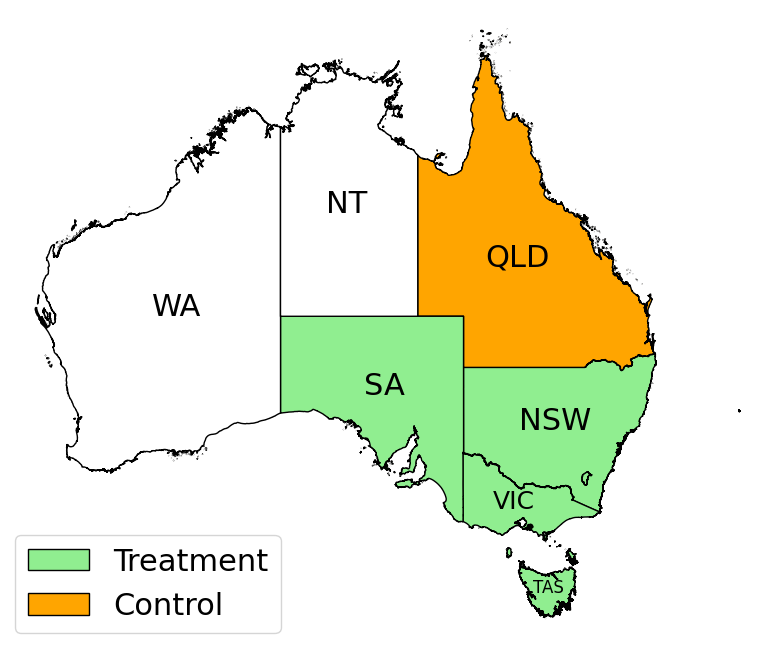
\includegraphics[width=0.4\textwidth]{map.png}
    \caption{Map of Australia showing treatment and control regions}
    \label{fig:map}
\end{figure}

\begin{figure}[ht]
    \centering
    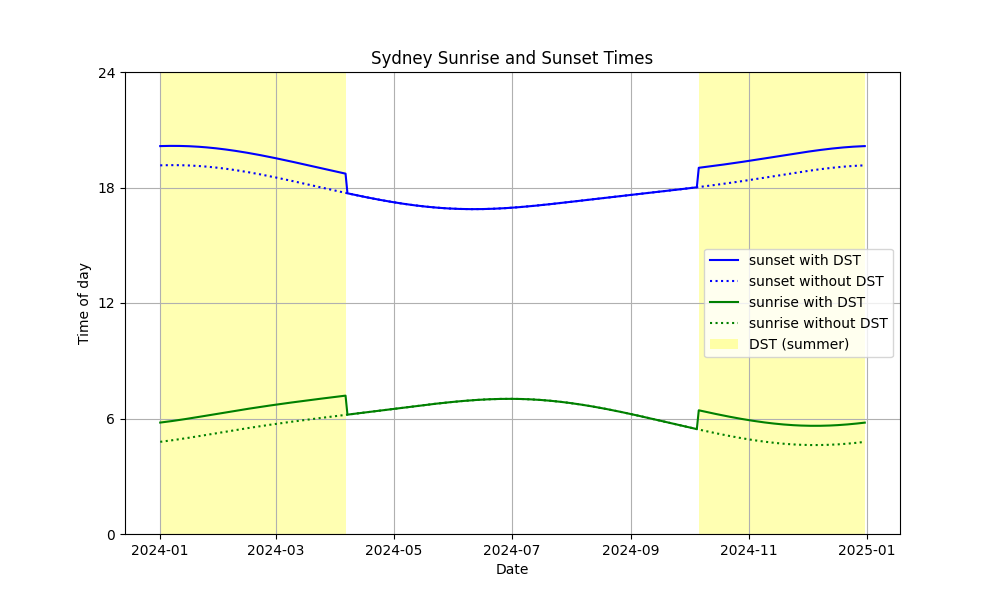
\includegraphics[width=\textwidth]{sunrise.png}
    \caption[Effect of \acs{DST} on apparent sunrise and sunset times in Sydney]{Effect of \acs{DST} on apparent sunrise and sunset times in Sydney. Note that since Australia is in the southern hemisphere, summer and \acs{DST} occur at the start and end of the calendar year.}
    \label{fig:sunrise plot}
\end{figure}

\begin{figure}[ht]
    \centering
    \begin{subfigure}[t]{0.45\textwidth} 
        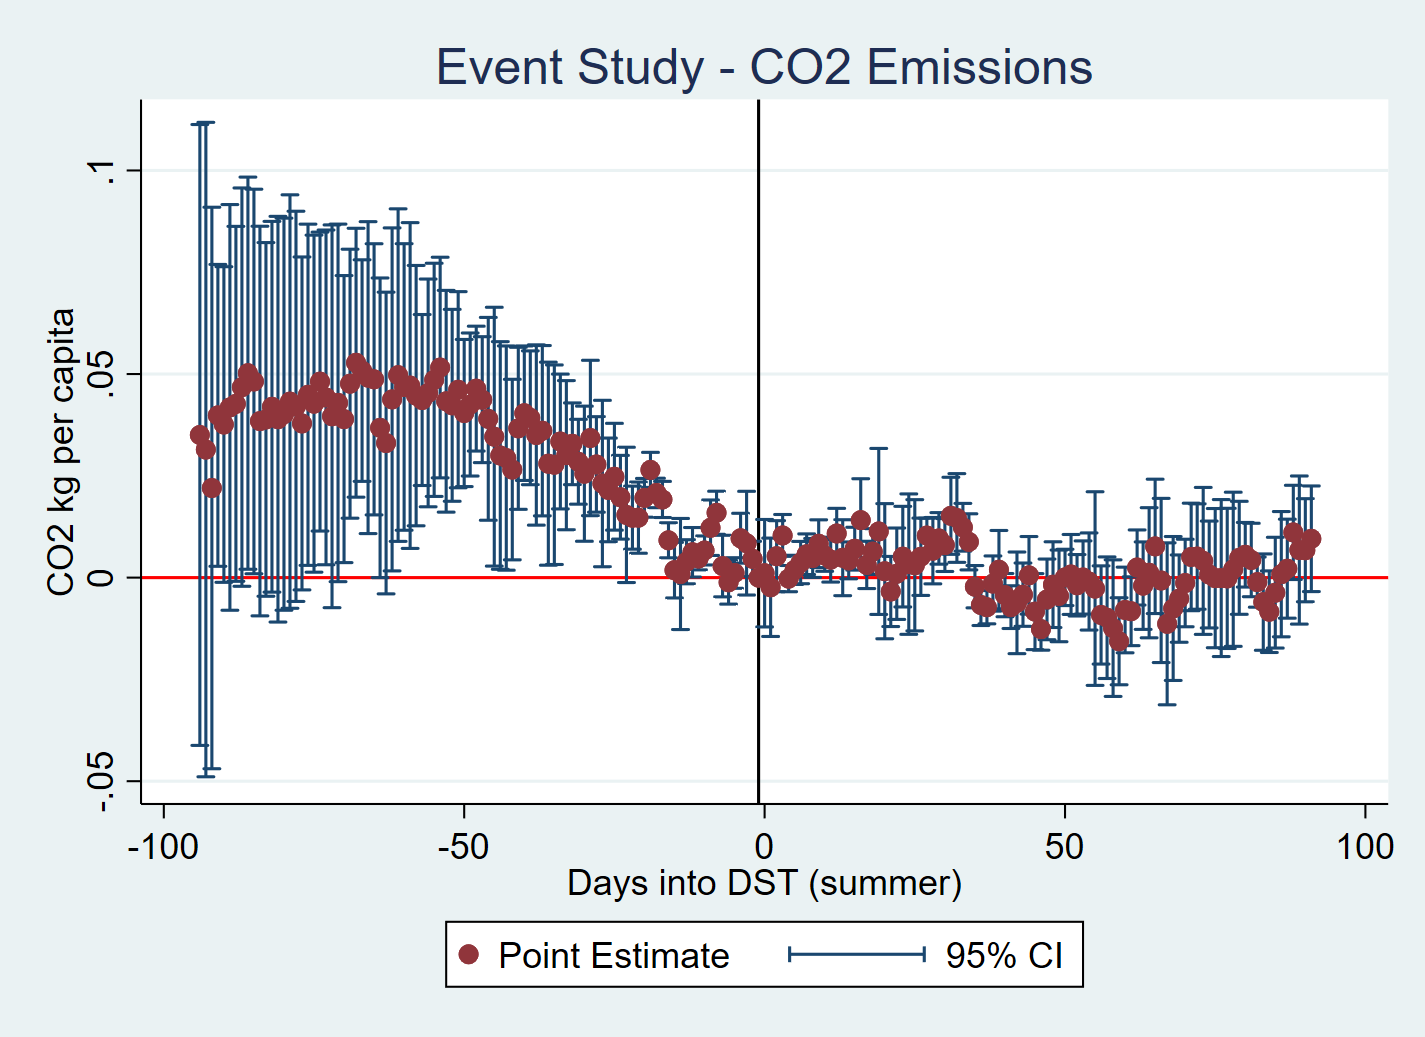
\includegraphics[width=\textwidth]{EventStudy-CO2.png}
        % Subcaption for the first image
        \caption{\acs{DiD} Event study plot for CO2 Emissions}
        \label{fig:dd event study co2}
    \end{subfigure}
    \hfill 
    \begin{subfigure}[t]{0.45\textwidth} 
        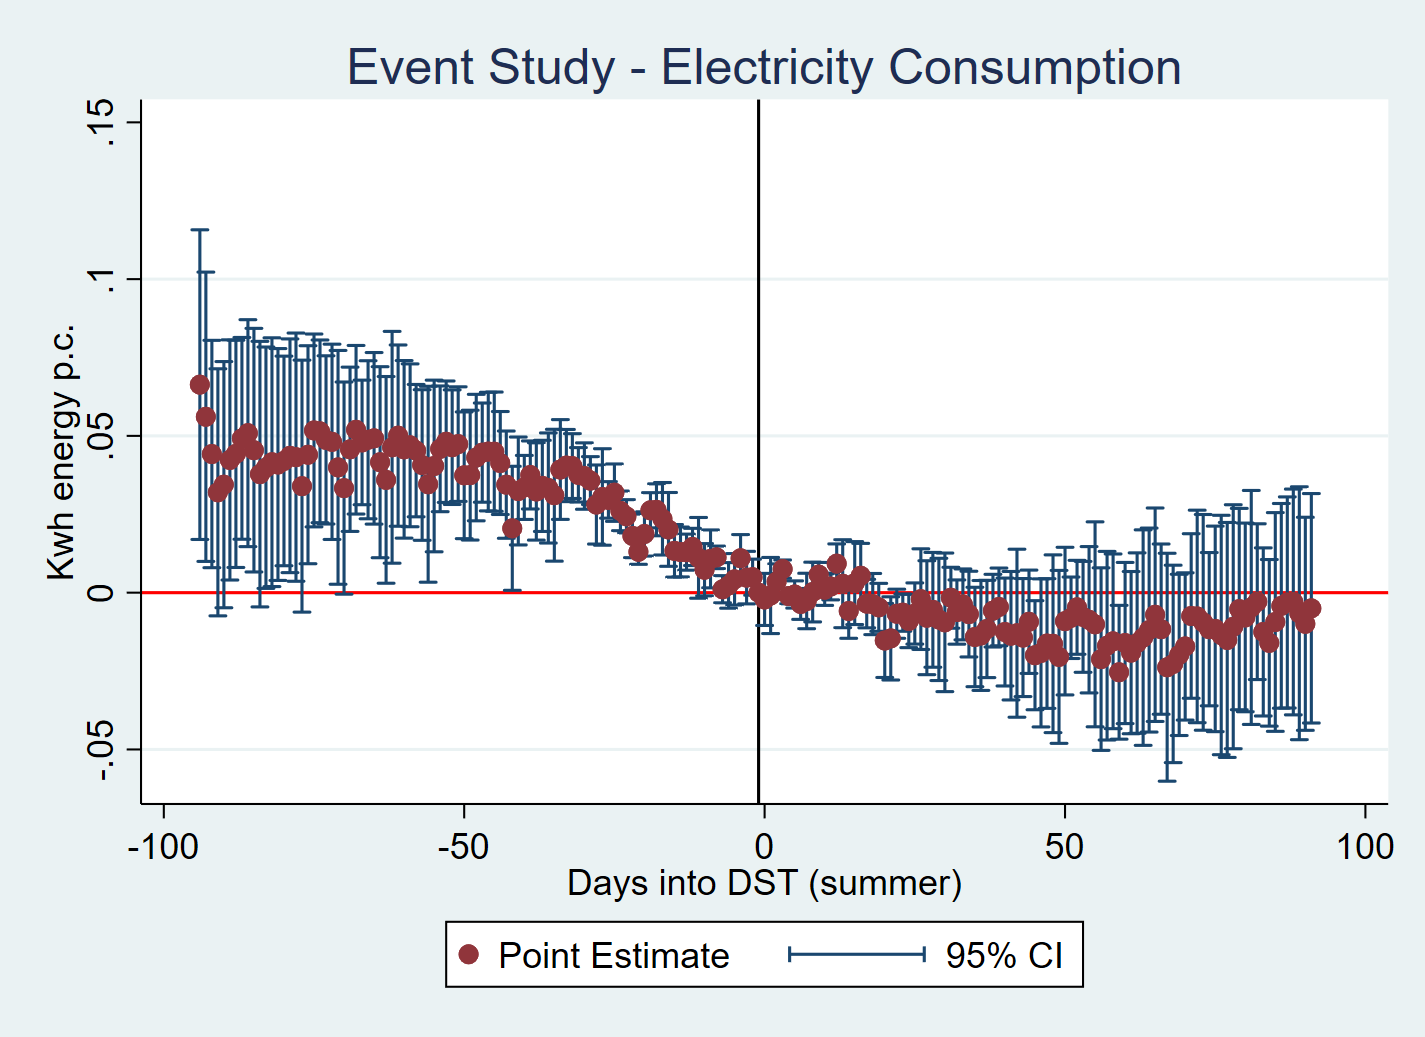
\includegraphics[width=\textwidth]{EventStudy-Elec.png} 
        \caption{\acs{DiD} Event study plot for CO2 Emissions} % Subcaption for the second image
        \label{fig:dd event study elec}
    \end{subfigure}
    % Shared caption for both subfigures
   \caption[Event study plots for \acs{DiD}]{Event study plots for \acs{DiD}. Both forward and backward clock changes are represented on the same plot, with the latter flipped accordingly. Summer is on the right of each plot, winter on the left. A common prior trend does not exist, because the points on the left half of each plot are jointly significant. The right half of each plot is close to zero, suggesting some sort of common post trend. However this is the treatment period, so such a result cannot be used to justify a \ac{DiD} to the control region.}
    \label{fig:dd event study}
\end{figure}


\begin{figure}[ht]
    \centering
    \begin{subfigure}[t]{0.45\textwidth} 
        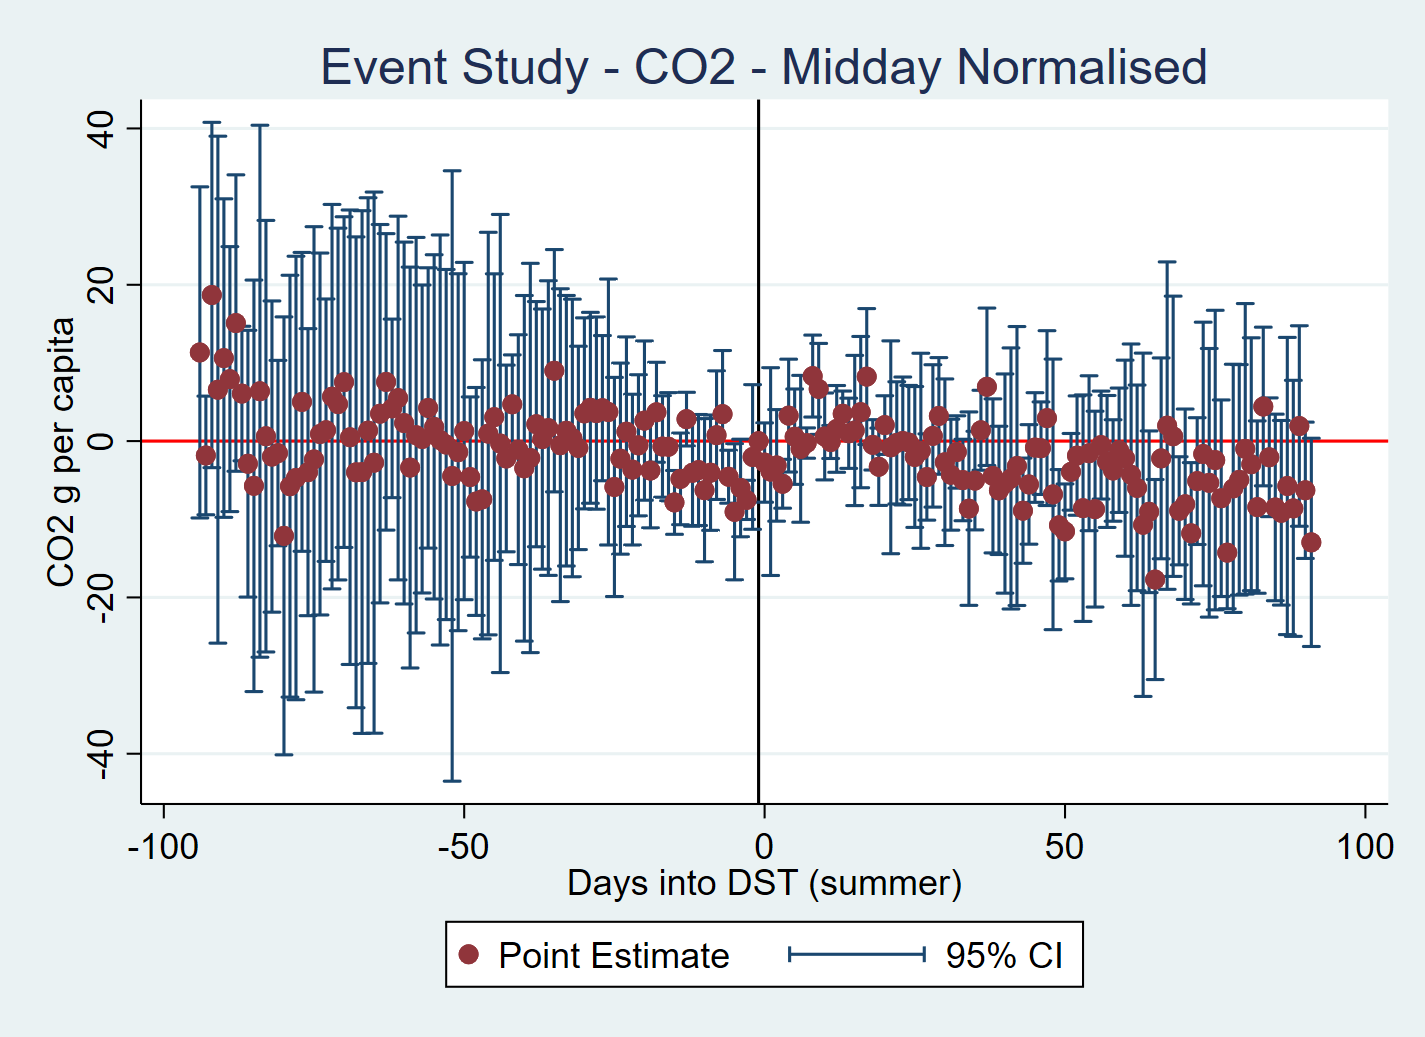
\includegraphics[width=\textwidth]{EventStudy-MiddayCO2.png}
        % Subcaption for the first image
        \caption{\acs{DDD} Event study plot for CO2 Emissions}
        \label{fig:ddd event study co2}
    \end{subfigure}
    \hfill 
    \begin{subfigure}[t]{0.45\textwidth} 
        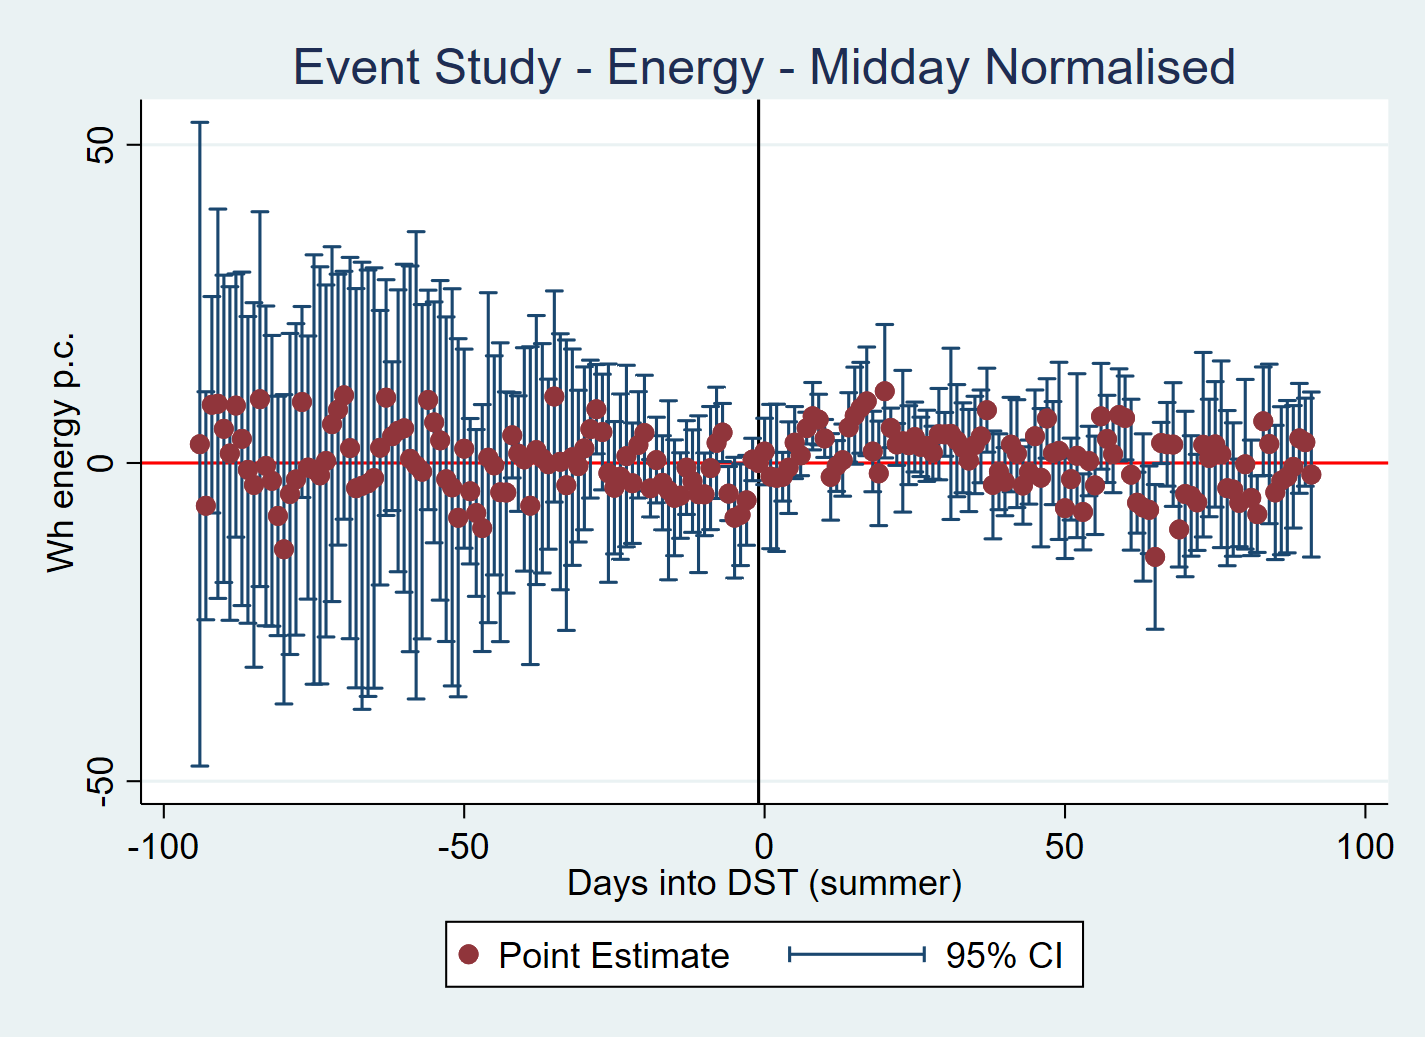
\includegraphics[width=\textwidth]{EventStudy-MiddayElec.png} 
        \caption{\acs{DDD} Event study plot for CO2 Emissions} % Subcaption for the second image
        \label{fig:ddd event study elec}
    \end{subfigure}
    % Shared caption for both subfigures
    \caption[Event study plots for \acs{DiD}]{Event study plots for \acs{DiD}. For each day, for each region, the average value of emission or energy during 12:00-14:30 was calculated, and subtracted from the value for all intervals. Then the same procedure was applied as for Figure \ref{fig:dd event study}. The left half of each plot is approximately zero, so there is a common prior trend. The right half is approximately zero, so there is a null result.} 
    \label{fig:ddd event study}
\end{figure}


\begin{figure}[ht]
    \centering
    \begin{subfigure}[t]{0.45\textwidth} 
        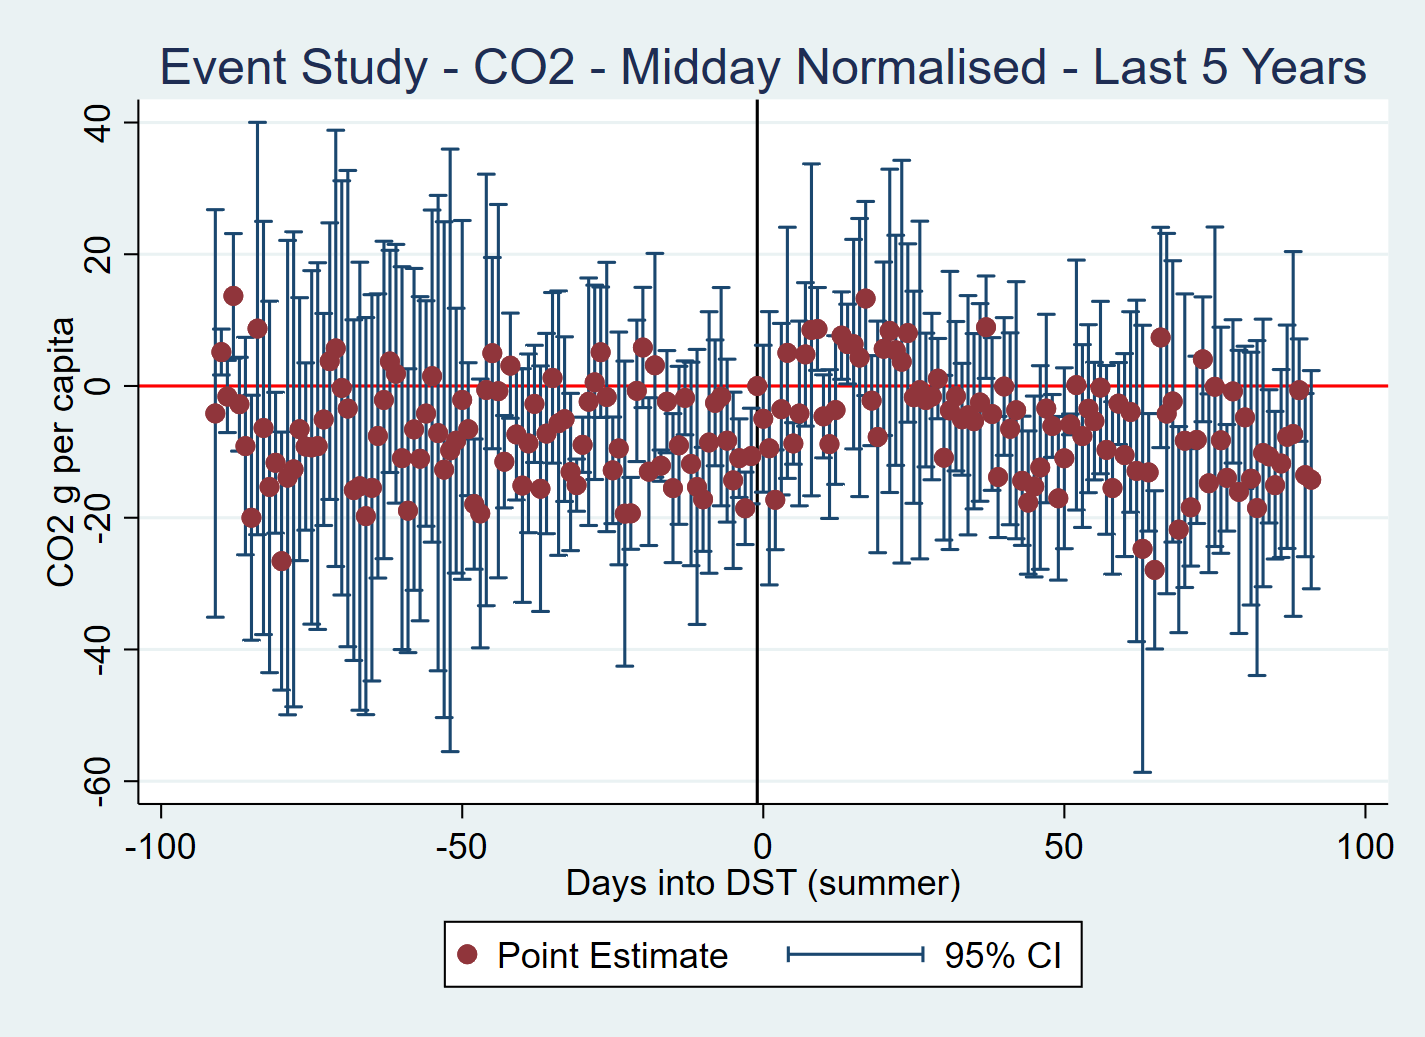
\includegraphics[width=\textwidth]{EventStudy-MiddayCO2-5year.png}
        % Subcaption for the first image
        \caption{\acs{DDD} Event study plot for CO2 Emissions - Last 5 years}
        \label{fig:ddd event study co2 - Last 5}
    \end{subfigure}
    \hfill 
    \begin{subfigure}[t]{0.45\textwidth} 
        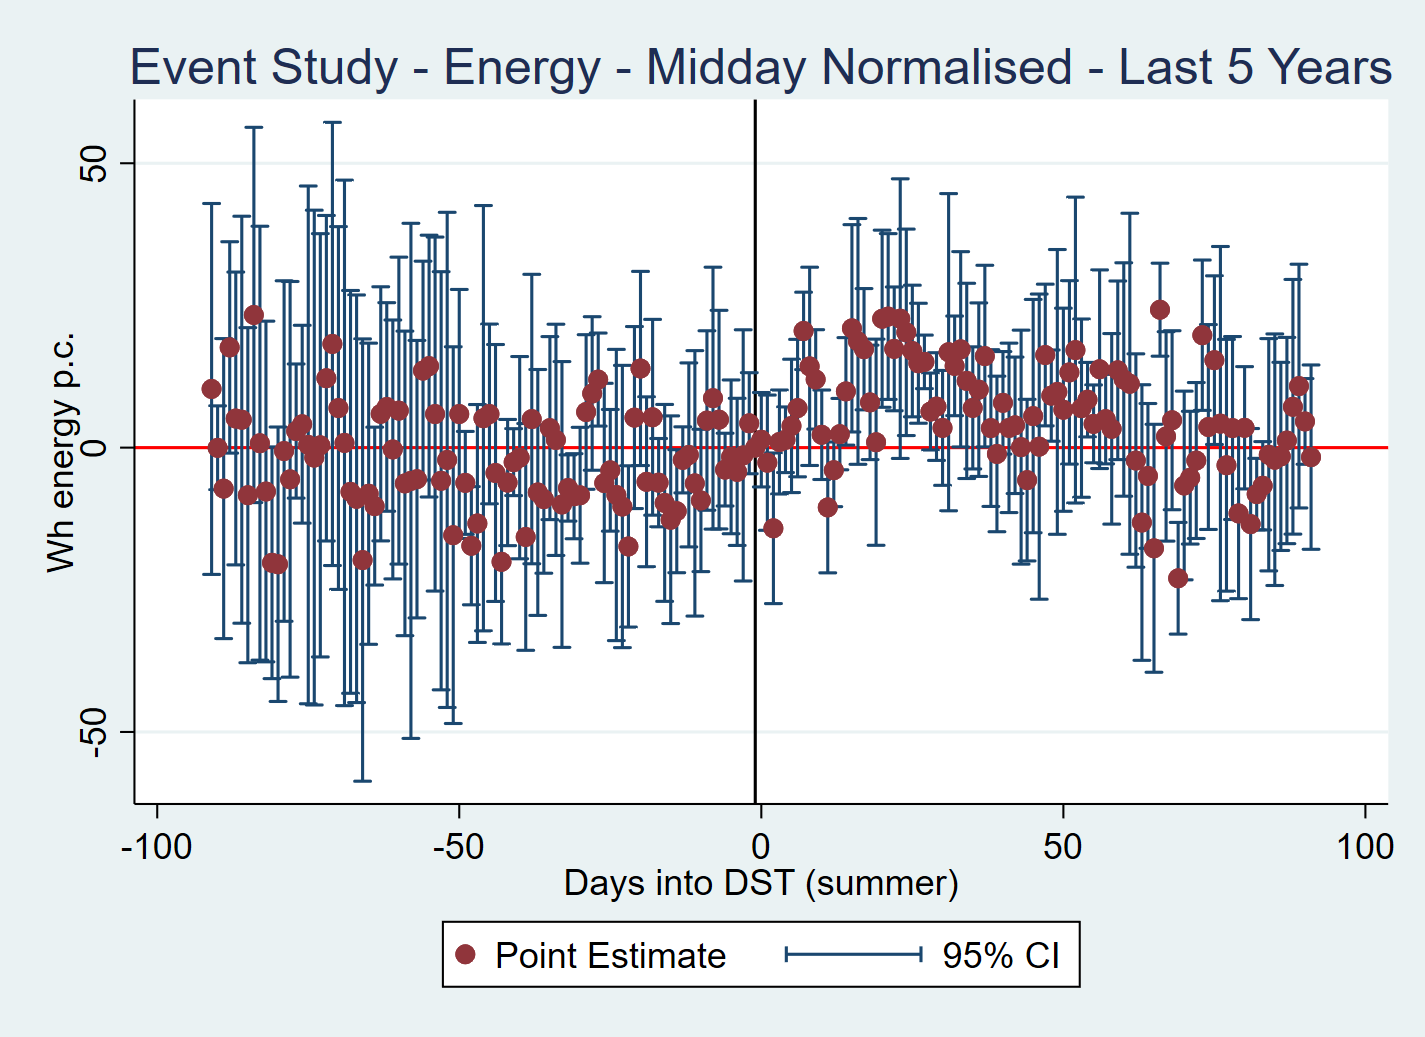
\includegraphics[width=\textwidth]{EventStudy-MiddayElec-5year.png} 
        \caption{\acs{DDD} Event study plot for Electricity consumption - Last 5 years} % Subcaption for the second image
        \label{fig:ddd event study elec - Last 5}
    \end{subfigure}
    % Shared caption for both subfigures
    \caption[Event study plots for \acs{DDD} using last 5 years]{Event study plots for \acs{DDD}. Using only the last 5 years of our data we see the size of our coefficients increase relative to the errors. However, our DDD regression results still remain insignificant at the 5\% level. \ref{DDD-Last-5-Results}} 
    \label{fig:ddd event study - Last 5}
\end{figure}

\begin{figure}[ht]
    \centering
    \begin{subfigure}[t]{0.45\textwidth} 
        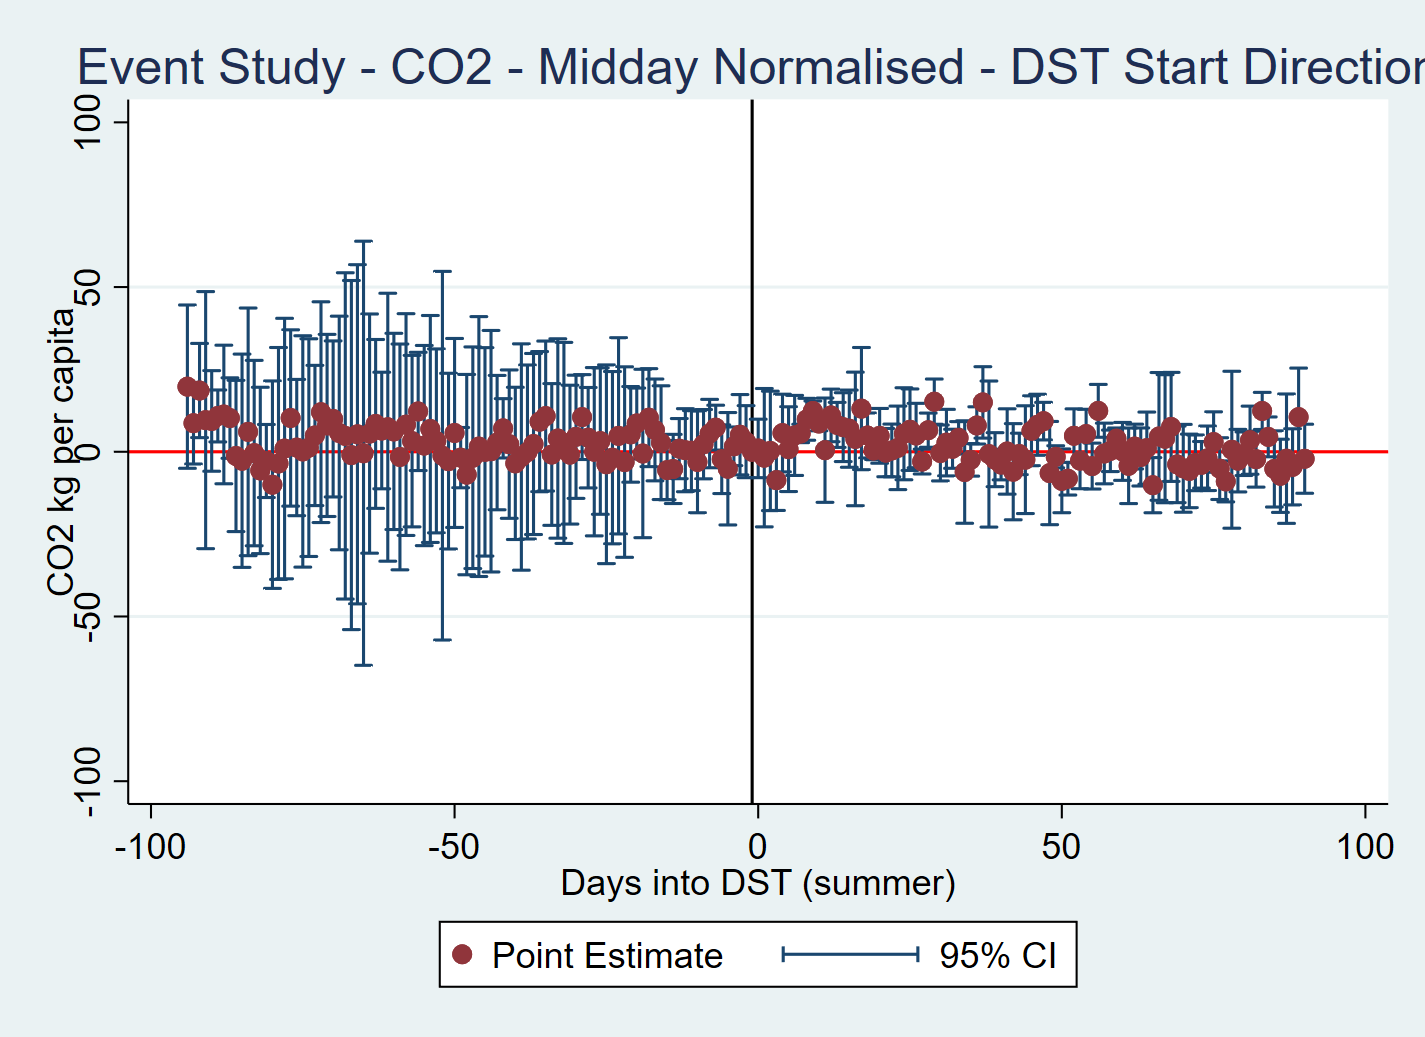
\includegraphics[width=\textwidth]{EventStudy-MiddayCO2-DST-Start.png}
        % Subcaption for the first image
        \caption{\acs{DDD} Event study plot for CO2 Emissions only for the DST start (clock forward)}
        \label{fig:ddd event study co2 start}
    \end{subfigure}
    \hfill 
    \begin{subfigure}[t]{0.45\textwidth} 
        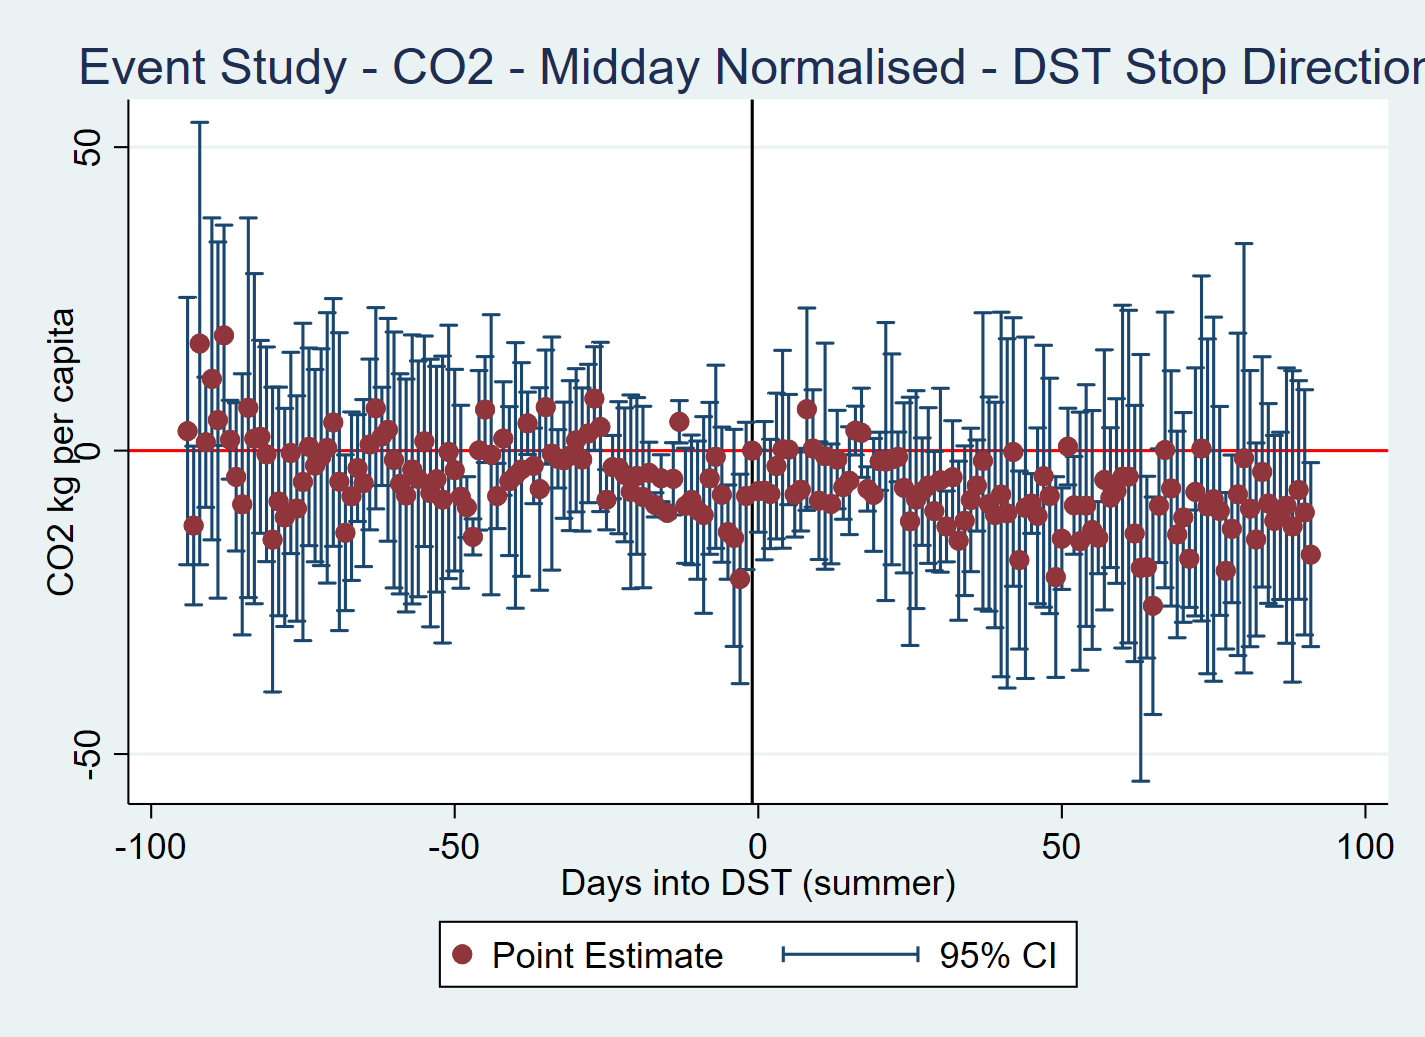
\includegraphics[width=\textwidth]{EventStudy-MiddayCO2-DST-Stop.png}
        \caption{\acs{DDD} Event study plot for CO2 Emissions only for the DST stop (clock backward). The plot chronologically reversed. The data starts in the middle of summer, during \acs{DST} on the right of the plot, and time progresses forwards towards the left. The clocks are moved back on the morning of day -1. Then once the treatment is unapplied, the ``Days into \acs{DST}" continues to become more negative, with mid-winter on the far left.} % Subcaption for the second image
        \label{fig:ddd event study co2 stop}
    \end{subfigure}
    % Shared caption for both subfigures
    \caption[Event study plots for \acs{DiD} split by clock change direction]{Event study plots for \acs{DiD}, split by clock direction. This is the same as Figure \ref{fig:ddd event study co2}, but split into clock forward and clock back transitions, as a robustness check. The common prior trend and null result still hold.} 
    \label{fig:ddd event study co2 start stop}
\end{figure}

\begin{figure}[ht]
    \centering
    \begin{subfigure}[t]{0.45\textwidth} 
        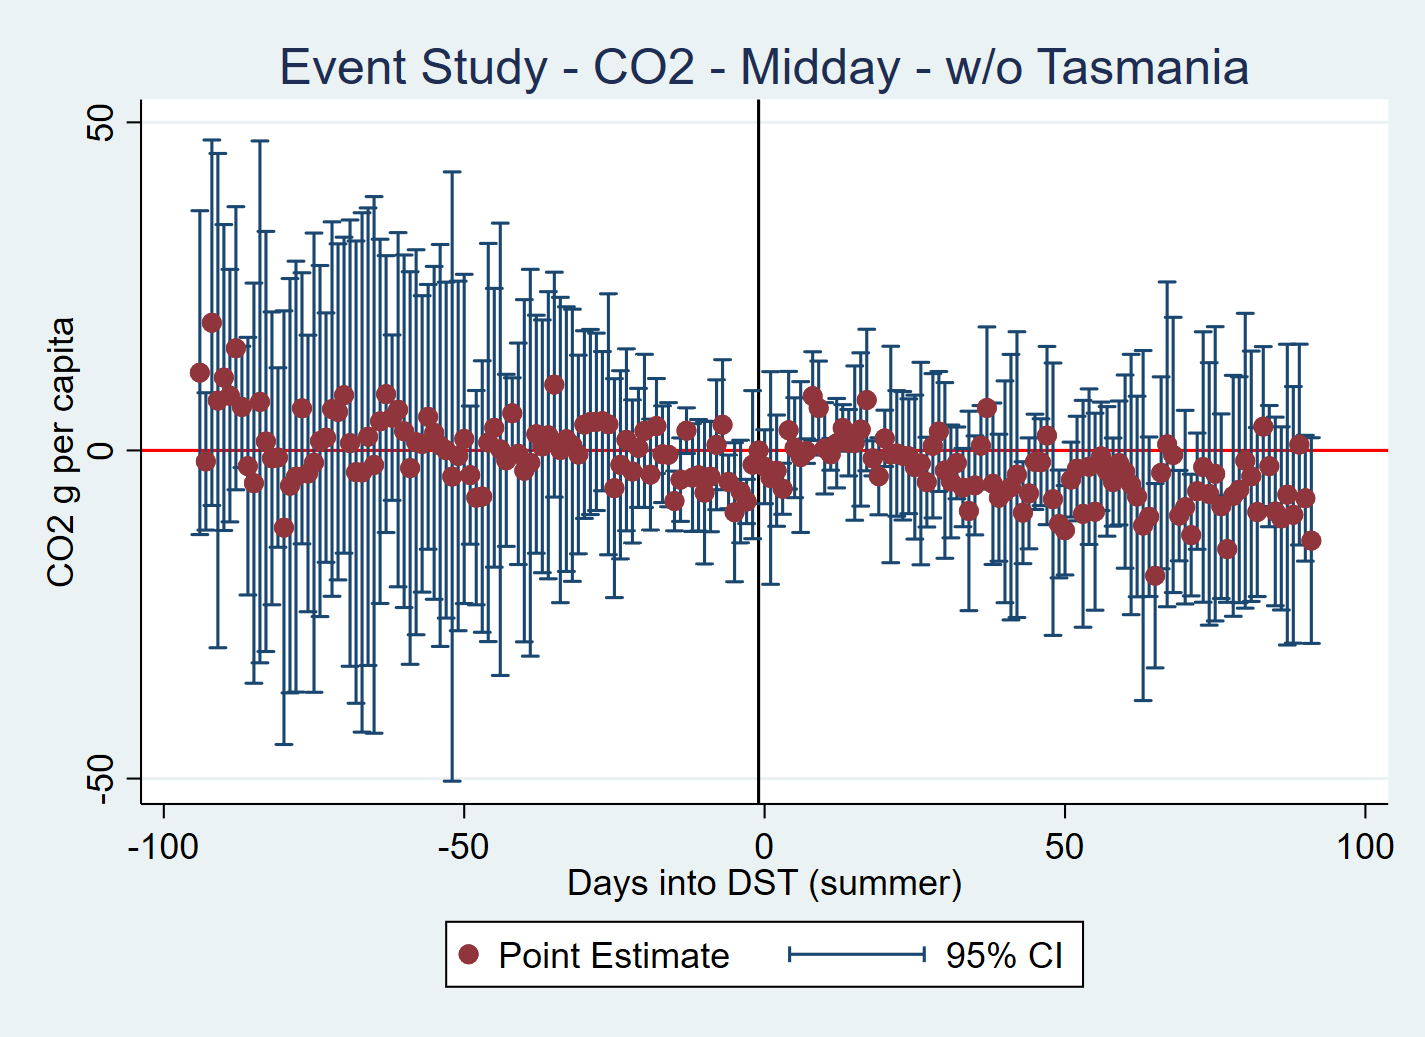
\includegraphics[width=\textwidth]{EventStudy-MiddayCO2-Dropping-Tasmania.png}
        % Subcaption for the first image
        \caption{\acs{DDD} Event study plot for CO2 Emissions when normalising for midday values and dropping Tasmania}
        \label{fig:ddd event study co2 w/o Tas}
    \end{subfigure}
    \hfill 
    \begin{subfigure}[t]{0.45\textwidth} 
        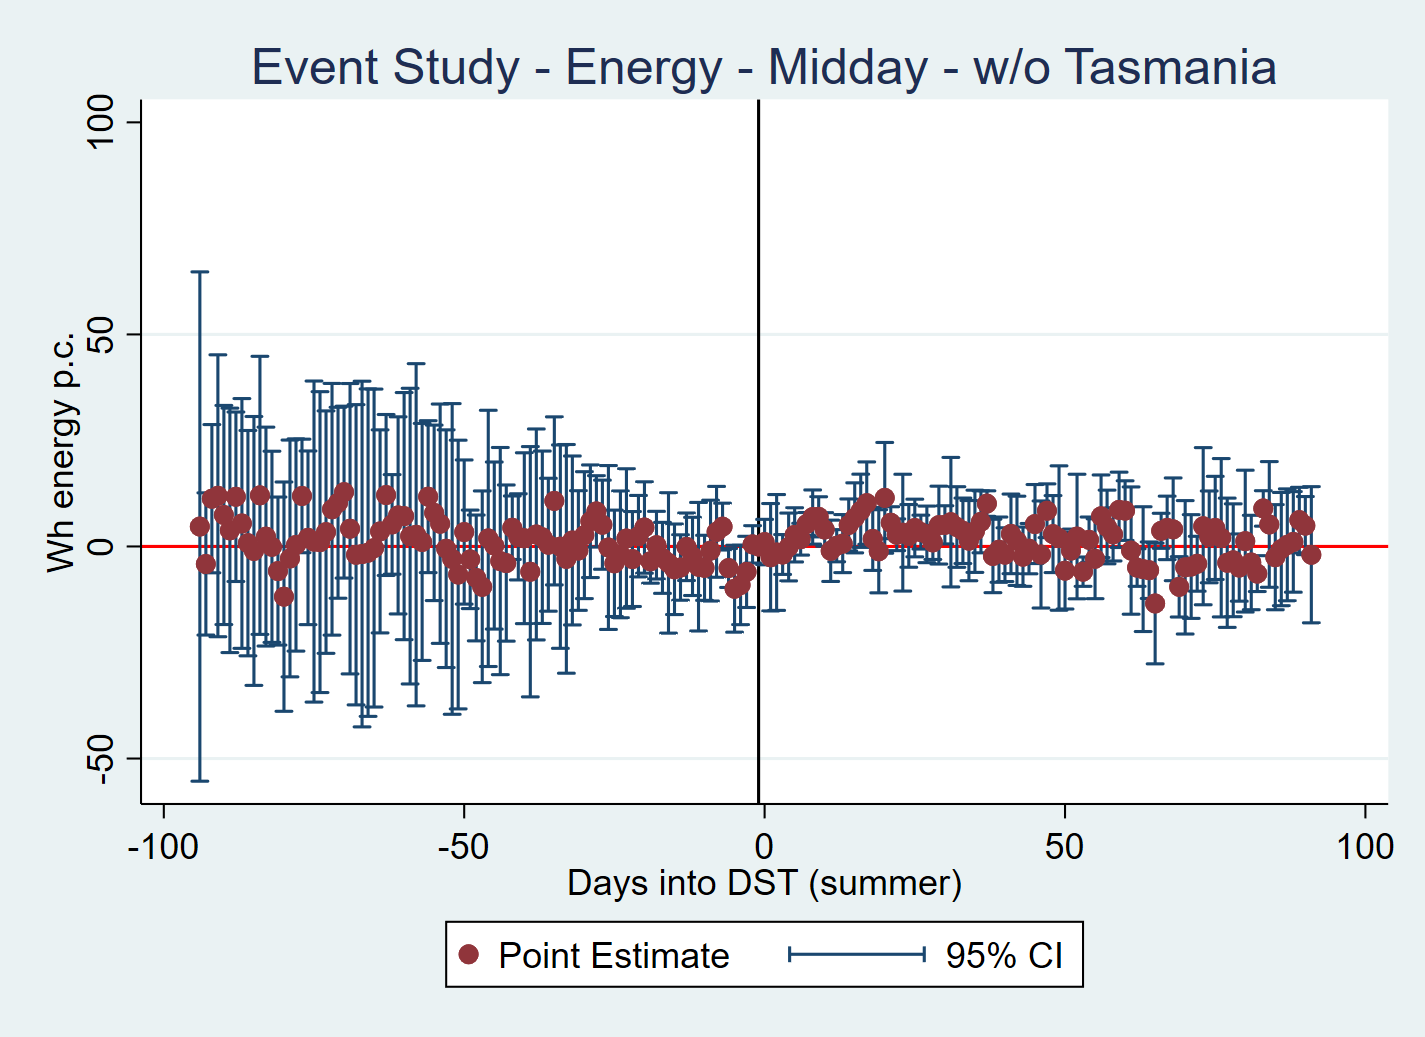
\includegraphics[width=\textwidth]{EventStudy-MiddayElec-Dropping-Tasmania.png}
        \caption{\acs{DDD} Event study plot for Electricity consumption when normalising for midday values and dropping Tasmania} % Subcaption for the second image
        \label{fig:ddd event study Elec w/o Tas}
    \end{subfigure}
    % Shared caption for both subfigures
    \caption[Event study plots for \acs{DDD} without Tasmania]{Event study plots for \acs{DDD}, dropping Tasmania as a robustness check. The common prior trend and null result still hold.} 
    \label{fig:ddd event study w/o Tas}
\end{figure}


\begin{figure}[ht]
    \centering
    \begin{subfigure}[t]{0.45\textwidth} 
        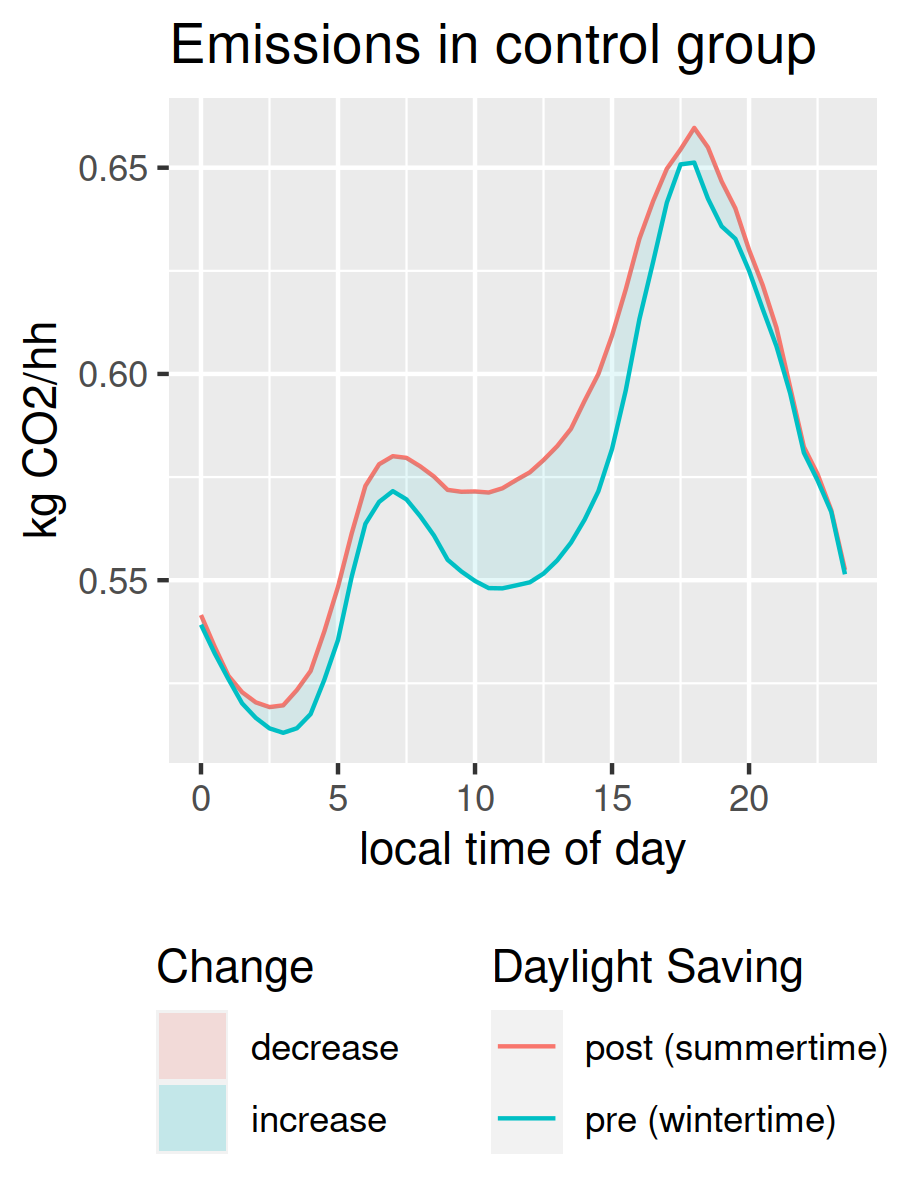
\includegraphics[width=\textwidth]{Images/intraday/co2_kg_per_capita/by-treated/control/hr_local-filled.png}
        % Subcaption for the first image
        \caption{Average intraday emissions in the control region}
        \label{fig:intraday co2 control}
    \end{subfigure}
    \hfill 
    \begin{subfigure}[t]{0.45\textwidth} 
        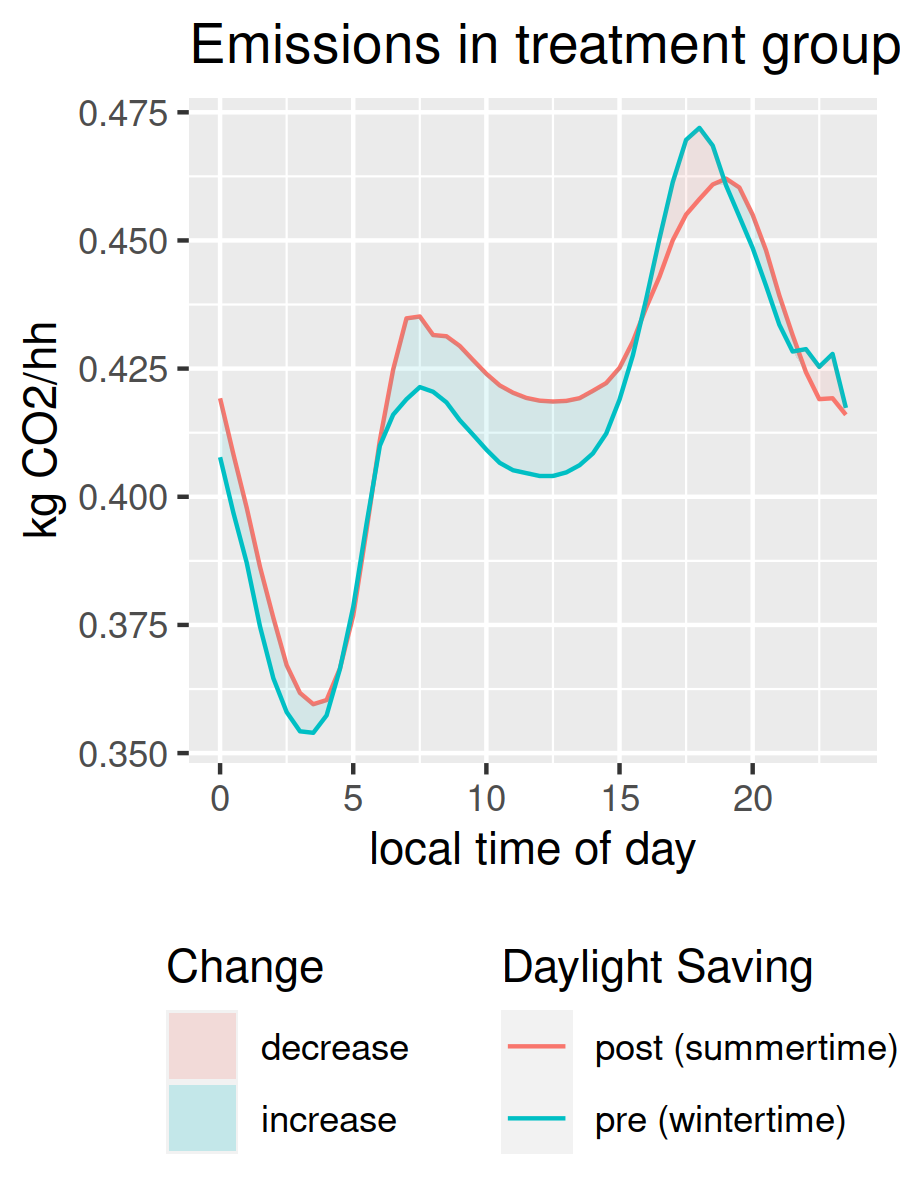
\includegraphics[width=\textwidth]{Images/intraday/co2_kg_per_capita/by-treated/treatment/hr_local-filled.png}
        \caption{Average intraday emissions in the treated regions} % Subcaption for the second image
        \label{fig:intraday co2 treated}
    \end{subfigure}
    % Shared caption for both subfigures
    \caption[Average intraday emissions, with and without \acs{DST}, for treated and control]{Average intraday emissions, with and without \acs{DST}, for treated and control. The fact that there is more of the red (decrease) area and less of the green (increase) for the treated region than the control suggests that \acs{DST} does reduce emissions. However this effect disappears once accounting for controls.} 
    \label{fig:intraday co2}
\end{figure}


\begin{figure}[ht]
    \centering
    \begin{subfigure}[t]{0.45\textwidth} 
        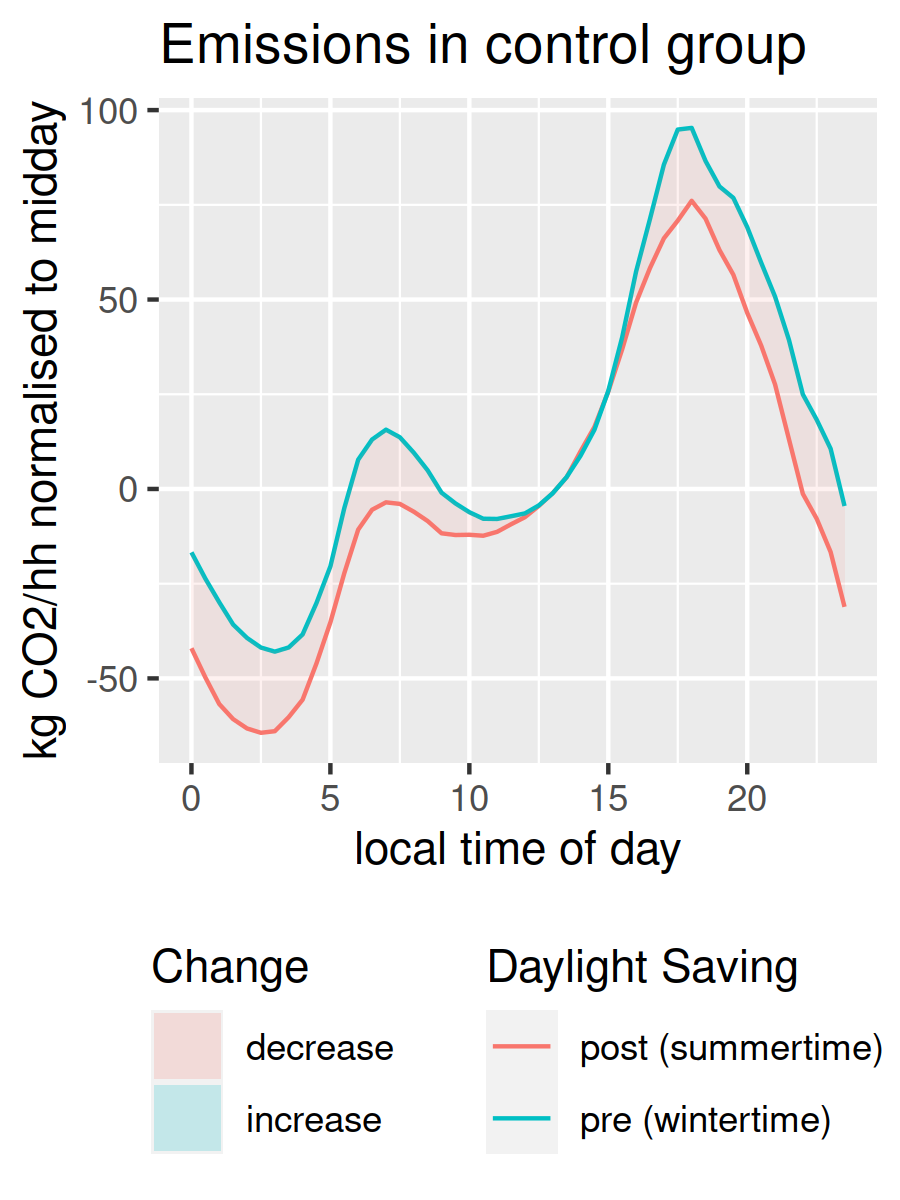
\includegraphics[width=\textwidth]{Images/intraday/co2_g_per_capita_vs_midday/by-treated/control/hr_local-filled.png}
        % Subcaption for the first image
        \caption{Average intraday emissions in the control region}
        \label{fig:intraday co2 control midday}
    \end{subfigure}
    \hfill 
    \begin{subfigure}[t]{0.45\textwidth} 
        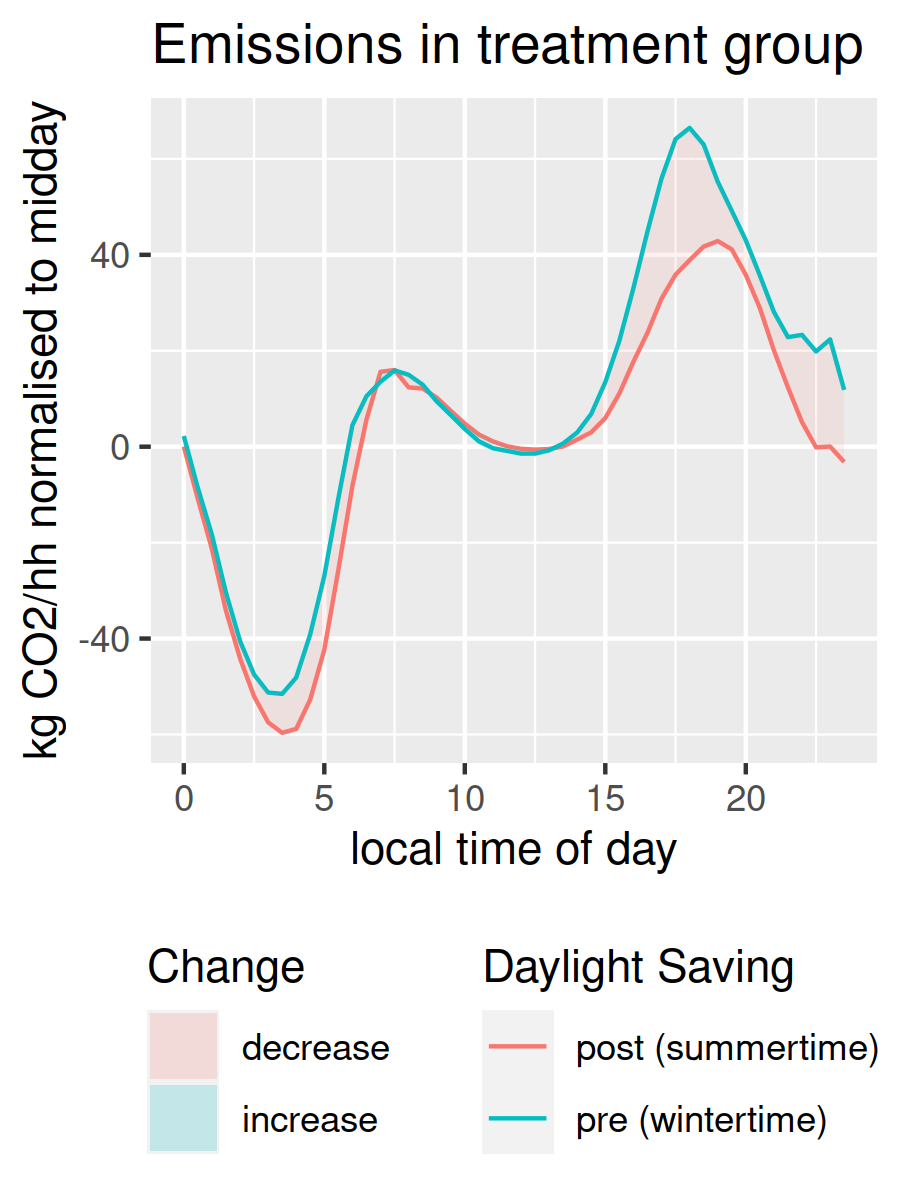
\includegraphics[width=\textwidth]{Images/intraday/co2_g_per_capita_vs_midday/by-treated/treatment/hr_local-filled.png}
        \caption{Average intraday emissions in the treated regions} % Subcaption for the second image
        \label{fig:intraday co2 treated midday}
    \end{subfigure}
    % Shared caption for both subfigures
    \caption[Average intraday emissions, normalising for midday]{Average intraday emissions, normalising for midday. This is the same as Figure \ref{fig:intraday co2}, except the average of the emissions for that day for that region was calculated for 12:00-14:30, and that was subtracted from all intervals for that day. This graphically represents the third differencing step. The fact that the red area (decrease) is larger for the control group suggests that \acs{DST} increases emissions. However once controls are accounted for in the regression, this difference changes sign and becomes statistically insignificant.} 
    \label{fig:intraday co2 midday}
\end{figure}



\begin{landscape}
 \begin{table}[!htbp] \centering
 \caption[Summary Statistics]{\label{tab:summary stats}Summary statistics for all variables, for treatment and control states}
 \begin{tabular}{@{\extracolsep{5pt}}clrccc}
 \hline \hline
    &&&&&\\ [-1.8ex]
  & \multicolumn{1}{l}{Variable} & \multicolumn{1}{r}{[unit]} & \multicolumn{1}{c}{Mean} & \multicolumn{1}{c}{Minimum Value} & \multicolumn{1}{c}{Maximum Value}\\
 \hline
  \parbox[t]{2mm}{\multirow{12}{*}{\rotatebox[origin=l]{90}{\textbf{Treatment}}}}&&&&&\\ [-1.8ex]
   &Population& \([inhabitans]\)& 4,127,718& 505,468 & 8,806,160\\
 &&&&&\\
  &Greenhouse gas emissions per capita& \([kg/half hour]\))& 0.315 & 0.000 & 0.935\\[-1.8ex]
  &&&&&\\
 &Energy production per capita & \([kWh/half hour]\) & 0.533 & 0.001 &41.719\\[-1.8ex]
  &&&&&\\
&Temperature & \([^{\circ}C]\) & 20.97 & 7.20 &46.40\\[-1.8ex]
  &&&&&\\
 &Solar exposure& \([kWh/m^2]\) & 4.75 & 0.11& 9.80\\[-1.8ex]
  &&&&&\\
 &Wind& \([km/h]\) & 16.09 & 0.00 & 51.50\\[-1.8ex]
  &&&&&\\
 &Holiday& \([\% of days]\) &3.41 &3.15 &3.57\\[-1.8ex]
  &&&&&\\
 &Weekend& \([\% of days]\) &0.29&&\\
 \hline
  \parbox[t]{2mm}{\multirow{12}{*}{\rotatebox[origin=l]{90}{\textbf{Control}}}}&&&&&\\ [-1.8ex]
   &Population& \([inhabitans]\)&4,870,395 &4,350,135 &5,459,413\\
  &&&&&\\
 &Greenhouse gas emissions per capita& \([kg/half hour]\)& 0.591 & 0.277 & 0.911\\[-1.8ex]
  &&&&&\\
    &Energy production per capita & \([kWh/half hour]\) & 0.656 & 0.375 & 1.027\\[-1.8ex]
  &&&&&\\
 &Temperature & \([^{\circ}C]\) & 26.64 & 12.60& 41.20\\[-1.8ex]
  &&&&&\\
 &Solar exposure& \([kWh/m^2]\) & 6.13 & 0.50 & 9.27 \\[-1.8ex]
  &&&&&\\
 &Wind& \([km/h]\) & 16.37 & 3.60 &41.00\\[-1.8ex]
  &&&&&\\
 &Holiday& \([\% of days]\) &3.27& 3.27& 3.27\\[-1.8ex]
  &&&&&\\
 &Weekend& \([\% of days]\) &0.29&&\\[-1.8ex]
  &&&&&\\
 \hline
 \end{tabular}
 \end{table}
 \end{landscape}

\def\sym#1{\ifmmode^{#1}\else\(^{#1}\)\fi}

\begin{table}[!htbp] \centering 
  \caption{CO2 and Electricity Consumption Results - DiD} 
  \label{Main-DiD-Results} 
\small 
\def\sym#1{\ifmmode^{#1}\else\(^{#1}\)\fi}
\begin{tabular}{l*{4}{c}}
\\[-1.8ex]\hline 
\hline \\[-1.8ex] 
 & \multicolumn{4}{c}{\textit{Dependent variable:}} \\ 
\cline{2-5} 
\\[-1.8ex] &\multicolumn{1}{c}{kg CO2 p.c.}&\multicolumn{1}{c}{kWh energy p.c.}&\multicolumn{1}{c}{Kg CO2 p.c.}&\multicolumn{1}{c}{kWh energy p.c.}\\ 
\\[-1.8ex] & \multicolumn{1}{c}{(1)} & \multicolumn{1}{c}{(2)} & \multicolumn{1}{c}{(3)} & \multicolumn{1}{c}{(4)}\\ 
\hline \\[-1.8ex] 
Treatment &      -0.133\sym{*}  &      -0.180\sym{**} &      -0.144\sym{**} &      -0.215\sym{***}\\
                    &    (0.0391)         &    (0.0284)         &    (0.0281)         &    (0.0198)         \\
[1em]
Post &      0.0243\sym{***}&      0.0317\sym{***}&      0.0263         &      0.0315         \\
                    &  (1.50e-14)         &  (6.03e-15)         &    (0.0174)         &    (0.0174)         \\
[1em]
Treatment $\times$ Post &     -0.0330\sym{**} &     -0.0568\sym{**} &     -0.0181         &     -0.0235         \\
                    &   (0.00663)         &   (0.00920)         &    (0.0222)         &    (0.0161)         \\
[1em]
Weekend &                     &                     &     -0.0338\sym{***}&     -0.0462\sym{***}\\
                    &                     &                     &   (0.00132)         &   (0.00181)         \\
[1em]
Public Holiday &                     &                     &     -0.0378\sym{**} &     -0.0498\sym{***}\\
                    &                     &                     &   (0.00556)         &   (0.00387)         \\
[1em]
Temperature &                     &                     &     -0.0109         &     -0.0250         \\
                    &                     &                     &    (0.0142)         &    (0.0168)         \\
[1em]
Temperature$^2$ &                     &                     &    0.000272         &    0.000521         \\
                    &                     &                     &  (0.000235)         &  (0.000289)         \\
[1em]
Solar Exposure &                     &                     &    -0.00422         &    -0.00815         \\
                    &                     &                     &   (0.00631)         &   (0.00600)         \\
[1em]
Wind$^3$ &                     &                     &     -0.0594         &     0.00417         \\
                    &                     &                     &    (0.0249)         &    (0.0119)         \\
[1em]
Constant            &       0.576\sym{***}&       0.656\sym{***}&       0.736\sym{*}  &       1.008\sym{*}  \\
                    &  (1.41e-14)         &  (6.97e-15)         &     (0.215)         &     (0.265)         \\
\hline
r2                  &       0.152         &       0.326         &       0.213         &       0.378         \\
r2\_a                &       0.152         &       0.326         &       0.213         &       0.378         \\
\hline\hline
\multicolumn{5}{l}{Note: Errors clustered by region, weighted by population.} \\
\multicolumn{2}{l}{Dependent variables are measured per half hour.} \\
\multicolumn{5}{l}{\footnotesize Standard errors in parentheses}\\
\multicolumn{5}{l}{\footnotesize \sym{*} \(p<0.05\), \sym{**} \(p<0.01\), \sym{***} \(p<0.001\)}\\
\end{tabular}
\end{table}

\def\sym#1{\ifmmode^{#1}\else\(^{#1}\)\fi}

\begin{table}[!htbp] \centering 
  \caption{Results For CO2 and Electricity Consumption DDD With Controls} 
  \label{Main-DDD-Results} 
\small 
\begin{tabular}{@{\extracolsep{5pt}}lD{.}{.}{-3} D{.}{.}{-3} } 
\\[-1.8ex]\hline 
\hline \\[-1.8ex] 
 & \multicolumn{2}{c}{\textit{Dependent variable:}} \\ 
\cline{2-3} 
\\[-1.8ex] & \multicolumn{1}{c}{Kg CO2 p.c.} & \multicolumn{1}{c}{Kwh energy consumption p.c.} \\ 
\\[-1.8ex] & \multicolumn{1}{c}{(1)} & \multicolumn{1}{c}{(2)}\\ 
\hline \\[-1.8ex]
Treatment&      -0.134\sym{*}  &      -0.216\sym{***}\\
                    &    (0.0306)         &    (0.0216)         \\
[1em]
Post&      0.0605\sym{*}  &      0.0788\sym{*}  \\
                    &    (0.0174)         &    (0.0174)         \\
[1em]
Treatment $\times$ Post &     -0.0303         &     -0.0401         \\
                    &    (0.0186)         &    (0.0196)         \\
[1em]
Not Midday &      0.0272\sym{***}&      0.0143\sym{***}\\
                    &  (8.78e-13)         &  (1.00e-12)         \\
[1em]
Treatment $\times$ Not Midday &     -0.0115         &    0.000875         \\
                    &   (0.00874)         &   (0.00608)         \\
[1em]
Post $\times$ Not Midday &     -0.0382\sym{***}&     -0.0529\sym{***}\\
                    &  (2.00e-12)         &  (2.33e-12)         \\
[1em]
Treatment $\times$ Post $\times$ Not Midday &      0.0136         &      0.0185         \\
                    &    (0.0129)         &    (0.0110)         \\
[1em]
Weekend    &     -0.0338\sym{***}&     -0.0462\sym{***}\\
                    &   (0.00132)         &   (0.00181)         \\
[1em]
Public Holiday &     -0.0378\sym{**} &     -0.0498\sym{***}\\
                    &   (0.00556)         &   (0.00387)         \\
[1em]
Temperature&     -0.0109         &     -0.0250         \\
                    &    (0.0142)         &    (0.0168)         \\
[1em]
Temperature2 &    0.000272         &    0.000521         \\
                    &  (0.000235)         &  (0.000289)         \\
[1em]
Solar Exposure&    -0.00422         &    -0.00815         \\
                    &   (0.00631)         &   (0.00600)         \\
[1em]
Wind3 &     -0.0594         &     0.00417         \\
                    &    (0.0249)         &    (0.0119)         \\
[1em]
Constant            &       0.712\sym{*}  &       0.995\sym{*}  \\
                    &     (0.215)         &     (0.265)         \\
\hline
r2                  &       0.214         &       0.380         \\
r2\_a                &       0.214         &       0.380         \\
\hline \\[-1.8ex] 
\hline 
\hline \\[-1.8ex] 
\multicolumn{2}{l}{Note: Errors clustered by region, weighted by population} \\ \multicolumn{2}{l}{$^{*}$p$<$0.1; $^{**}$p$<$0.05; $^{***}$p$<$0.01} \\ 
\end{tabular} 
\end{table} 
\def\sym#1{\ifmmode^{#1}\else\(^{#1}\)\fi}

\begin{table}[!htbp] \centering 
  \caption{Results For CO2 and Electricity Consumption Base DDD Without Controls} 
  \label{DDD-WO-Controls-Results} 
\small 
\begin{tabular}{@{\extracolsep{5pt}}lD{.}{.}{-3} D{.}{.}{-3} } 
\\[-1.8ex]\hline 
\hline \\[-1.8ex] 
 & \multicolumn{2}{c}{\textit{Dependent variable:}} \\ 
\cline{2-3} 
\\[-1.8ex] & \multicolumn{1}{c}{Kg CO2 p.c.} & \multicolumn{1}{c}{Kwh energy consumption p.c.} \\ 
\\[-1.8ex] & \multicolumn{1}{c}{(1)} & \multicolumn{1}{c}{(2)}\\ 
\hline \\[-1.8ex]
\hline
Treatment &      -0.123\sym{*}  &      -0.180\sym{**} \\
                    &    (0.0435)         &    (0.0256)         \\
[1em]
Post &      0.0585\sym{***}&      0.0790\sym{***}\\
                    &  (1.26e-13)         &  (2.01e-13)         \\
[1em]
Treatment $\times$ Post &     -0.0451\sym{***}&     -0.0734\sym{**} \\
                    &   (0.00506)         &    (0.0142)         \\
[1em]
Not Midday &      0.0272\sym{***}&      0.0143\sym{***}\\
                    &  (1.28e-13)         &  (1.27e-13)         \\
[1em]
Treatment $\times$ Not Midday &     -0.0115         &    0.000858         \\
                    &   (0.00875)         &   (0.00608)         \\
[1em]
Post $\times$ Not Midday &     -0.0382\sym{***}&     -0.0529\sym{***}\\
                    &  (1.67e-13)         &  (2.29e-13)         \\
[1em]
Treatment $\times$ Post $\times$ Not Midday &      0.0136         &      0.0185         \\
                    &    (0.0129)         &    (0.0110)         \\
[1em]
Constant            &       0.552\sym{***}&       0.643\sym{***}\\
                    &  (1.28e-13)         &  (1.34e-13)         \\
\hline
r2                  &       0.153         &       0.328         \\
r2\_a                &       0.153         &       0.328         \\
\hline\hline
\multicolumn{3}{l}{\footnotesize Standard errors in parentheses}\\
\multicolumn{3}{l}{\footnotesize \sym{*} \(p<0.05\), \sym{**} \(p<0.01\), \sym{***} \(p<0.001\)}\\
\end{tabular}
\end{table}
\def\sym#1{\ifmmode^{#1}\else\(^{#1}\)\fi}

\begin{table}[!htbp] \centering 
  \caption{Results For ln(CO2) and ln(Electricity Consumption) DDD With Controls} 
  \label{DDD-ln-Results} 
\small 
\begin{tabular}{@{\extracolsep{5pt}}lD{.}{.}{-3} D{.}{.}{-3} } 
\\[-1.8ex]\hline 
\hline \\[-1.8ex] 
 & \multicolumn{2}{c}{\textit{Dependent variable:}} \\ 
\cline{2-3} 
\\[-1.8ex] & \multicolumn{1}{c}{ln(Kg CO2 p.c.)} & \multicolumn{1}{c}{ln(Kwh energy consumption p.c.)} \\ 
\\[-1.8ex] & \multicolumn{1}{c}{(1)} & \multicolumn{1}{c}{(2)}\\ 
\hline \\[-1.8ex]
Treatment &      -0.351\sym{*}  &      -0.409\sym{***}\\
                    &     (0.124)         &    (0.0464)         \\
[1em]
Post &       0.130         &       0.108\sym{*}  \\
                    &    (0.0509)         &    (0.0280)         \\
[1em]
Treatment $\times$ Post &     -0.0490         &     -0.0566         \\
                    &    (0.0524)         &    (0.0337)         \\
[1em]
Not Midday &      0.0569\sym{***}&      0.0224\sym{***}\\
                    &  (3.57e-12)         &  (1.43e-12)         \\
[1em]
Treatment $\times$ Not Midday &     0.00157         &      0.0116         \\
                    &    (0.0291)         &    (0.0131)         \\
[1em]
Post $\times$ Not Midday &     -0.0671\sym{***}&     -0.0764\sym{***}\\
                    &  (6.78e-12)         &  (3.25e-12)         \\
[1em]
Treatment $\times$ Post $\times$ Not Midday&      0.0186         &      0.0153         \\
                    &    (0.0311)         &    (0.0242)         \\
[1em]
Weekend &     -0.0774\sym{**} &     -0.0947\sym{***}\\
                    &    (0.0124)         &    (0.0109)         \\
[1em]
Public Holiday &     -0.0900\sym{*}  &      -0.110\sym{**} \\
                    &    (0.0226)         &    (0.0155)         \\
[1em]
Temperature &     -0.0178         &     -0.0402         \\
                    &    (0.0352)         &    (0.0225)         \\
[1em]
Temperature2 &    0.000501         &    0.000872         \\
                    &  (0.000578)         &  (0.000380)         \\
[1em]
Solar Exposure &     -0.0171         &     -0.0148         \\
                    &    (0.0204)         &   (0.00913)         \\
[1em]
Wind3 &      -0.205         &     0.00503         \\
                    &     (0.102)         &    (0.0206)         \\
[1em]
Constant            &      -0.278         &       0.111         \\
                    &     (0.525)         &     (0.366)         \\
\hline
r2                  &       0.171         &       0.400         \\
r2\_a                &       0.171         &       0.400         \\
\hline \\[-1.8ex] 
\hline 
\hline \\[-1.8ex] 
\multicolumn{2}{l}{Note: Errors clustered by region, weighted by population} \\ \multicolumn{2}{l}{$^{*}$p$<$0.1; $^{**}$p$<$0.05; $^{***}$p$<$0.01} \\ 
\end{tabular} 
\end{table} 

\def\sym#1{\ifmmode^{#1}\else\(^{#1}\)\fi}

\begin{table}[!htbp] \centering 
  \caption{Results For CO2 and Electricity Consumption DDD With Controls - Last 5 Years} 
  \label{DDD-Last-5-Results} 
\small 
\begin{tabular}{@{\extracolsep{5pt}}lD{.}{.}{-3} D{.}{.}{-3} } 
\\[-1.8ex]\hline 
\hline \\[-1.8ex] 
 & \multicolumn{2}{c}{\textit{Dependent variable:}} \\ 
\cline{2-3} 
\\[-1.8ex] & \multicolumn{1}{c}{Kg CO2 p.c.} & \multicolumn{1}{c}{Kwh energy consumption p.c.} \\ 
\\[-1.8ex] & \multicolumn{1}{c}{(1)} & \multicolumn{1}{c}{(2)}\\ 
\hline \\[-1.8ex]
Treatment&      -0.137\sym{*}  &      -0.209\sym{***}\\
                    &    (0.0324)         &    (0.0237)         \\
[1em]
Post &      0.0614\sym{*}  &      0.0747\sym{*}  \\
                    &    (0.0170)         &    (0.0176)         \\
[1em]
Treatment $\times$ Post &     -0.0609\sym{**} &     -0.0680\sym{*}  \\
                    &    (0.0128)         &    (0.0175)         \\
[1em]
Not Midday&      0.0792\sym{***}&      0.0472\sym{***}\\
                    &  (3.65e-13)         &  (5.65e-13)         \\
[1em]
Treatment $\times$ Not Midday &     -0.0311         &     0.00107         \\
                    &    (0.0168)         &   (0.00890)         \\
[1em]
Post $\times$ Not Midday&     -0.0355\sym{***}&     -0.0496\sym{***}\\
                    &  (5.61e-13)         &  (8.43e-13)         \\
[1em]
Treatment $\times$ Post $\times$ Not Midday &      0.0230         &      0.0322\sym{*}  \\
                    &    (0.0127)         &    (0.0115)         \\
[1em]
Weekend    &     -0.0263\sym{***}&     -0.0368\sym{***}\\
                    &   (0.00125)         &   (0.00167)         \\
[1em]
Public holiday &     -0.0288\sym{*}  &     -0.0407\sym{**} \\
                    &   (0.00777)         &   (0.00594)         \\
[1em]
Temperature&    -0.00144         &     -0.0216         \\
                    &    (0.0111)         &    (0.0168)         \\
[1em]
Temperature2 &    0.000112         &    0.000471         \\
                    &  (0.000184)         &  (0.000293)         \\
[1em]
Solar Exposure &    -0.00724         &    -0.00978         \\
                    &   (0.00641)         &   (0.00595)         \\
[1em]
Wind3 &     -0.0471         &      0.0152         \\
                    &    (0.0243)         &    (0.0128)         \\
[1em]
Constant            &       0.477\sym{*}  &       0.869\sym{*}  \\
                    &     (0.167)         &     (0.264)         \\
\hline
r2                  &       0.424         &       0.445         \\
r2\_a                &       0.424         &       0.445         \\
\hline \\[-1.8ex] 
\hline 
\hline \\[-1.8ex] 
\multicolumn{2}{l}{Note: Errors clustered by region, weighted by population} \\ \multicolumn{2}{l}{$^{*}$p$<$0.1; $^{**}$p$<$0.05; $^{***}$p$<$0.01} \\ 
\end{tabular} 
\end{table} 
\begin{table}

\caption[Energy and emissions near sunrise and sunset]{\label{tab:sunrise emissions stats}Energy and emissions near sunrise and sunset. Emissions intensity is lower when the sun is up, but the difference is not the same.}
\centering
\begin{tabular}[t]{lrrr}
\toprule
period of day & power (W per capita) & CO2 (g/h per capita) & CO2 Intensity (g / kWh)\\
\midrule
the hour before sunrise & 477 & 453 & 982\\

the hour after sunrise & 513 & 476 & 959\\

the hour before sunset & 577 & 520 & 929\\

the hour after sunset & 592 & 530 & 923\\

remainder of day & 506 & 468 & 952\\
\bottomrule
\end{tabular}
\end{table}


\FloatBarrier
\addcontentsline{toc}{subsection}{Appendix B: Data column explanation}
\subsection*{Appendix B: Data column explanation}

This section describes the dataset used, after all the joins, transformations and enrichment are performed.

For the independent variable, ($y$), there is:

\begin{description}
    \item[\texttt{co2\_kg\_per\_capita}] kilograms of $CO_2$ emitted, per capita in this region (accounting for population growth over time), within this time interval. (e.g. within half hour for the half-hour file, or within the day for the daily file.)
    \item[\texttt{energy\_kwh\_per\_capita}] kilowatt hours of energy consumer, per capita in this region (accounting for population growth over time). Note that rooftop solar is counted as negative load by AEMO. So 10kWh of load plus 3kWh of solar appears here is 7kWh.
\end{description}

For the dependent variables ($x$) there is:

\begin{description}
    \item[\texttt{regionid}] the geographical state, as per AEMO convention. (AEMO always ends region id with a \texttt{1}) This is a string enum/factor. Options are:
    \begin{description}
        \item[\texttt{QLD1}] Queensland (our control region)
        \item[\texttt{NSW1}] New South Wales. (This includes the Australian Capital Territory (ACT))
        \item[\texttt{VIC1}] Victoria
        \item[\texttt{SA1}] South Australia
        \item[\texttt{TAS1}] Tasmania
    \end{description}
    \item[\texttt{dst\_now\_anywhere}] ``post" - dummy variable - is there daylight saving in this time interval. Even in the control region this is true.
    \item[\texttt{dst\_here\_anytime}] ``treatment" - dummy variable -  is this a region which has daylight saving. True even if there is not daylight saving in this time interval. Note that this value changes at midnight, even though in theory \ac{DST} transitions happen at 2am or 3am. In practice everyone changes their clocks before going to bed, so we don't expect these 5 hours per year to introduce much error. It simplifies the code and graphs to think of the 'post' as applying to a whole date.
    \item[\texttt{dst\_now\_here}] treatment x post - dummy variable. True if there is daylight saving in this region, on this day
    \item[\texttt{midday\_control}] a dummy - true if this half hour falls within 12:00-14:30. This is used for the third difference in our \ac{DDD}. 12:00-14:30 was chosen to match \cite{kellogg_daylight_2008}. 12:00-14:30 is Queensland time (no \ac{DST}) not local time.
    \item[\texttt{midday\_control\_local}] Same as \texttt{midday\_control}, but calculated based on local time in this region
    
    \item[\texttt{days\_into\_dst}] How far are we into the daylight saving period?
    \begin{itemize}
       \item  On the day when the clocks are moved forward, this is 0. 
       \item  The day after the clocks moved forward, it is 1.
       \item  In the middle of summer it is around 90.
       \item  The day before clocks move back (the last day with daylight saving) this is 0
       \item  the day the clocks move back, this is -1
       \item  the day after the clocks move back, this is -2
       \item  in the middle of winter, this approximately -90
       \item  the day before the clocks move forward in spring, this is -1
    \end{itemize}
\end{description}

Our other time variables are:

\begin{description}
    \item[\texttt{Date}] the date of the observation. (First letter capitalised to avoid a namespace clash with R's \texttt{date} function)
    \item[\texttt{public\_holiday}] dummy variable for if this date is a public holiday in this region. 
    \item[\texttt{hh\_end}] The datetime of the end of this half hour (when we have one row per half hour). The timezone is Queensland time (UTC+10, Australia/Brisbane, no daylight saving) even if this row is for a different region.
    \item[\texttt{hh\_start}] the start of this half hour period
    \item[\texttt{dst\_date}] The date of the nearest daylight saving transition (which may be in the future or the past). Note that all treatment regions move their clocks on the same day. So the value is the same for all regions on a given day. Even for the control region (Queensland) this value is populated.
    \item[\texttt{dst\_direction}] A string factor/enum about the direction of the clock change at \texttt{dst\_date}. Either \texttt{start} (move clocks forward, in October, spring) or \texttt{stop} (move clocks back, in Autumn).
    \item[\texttt{dst\_transition\_id}] A unique string to represent each clock transition. e.g. \texttt{2009-start}, \texttt{2009-stop}. This is a string identifier for \texttt{dst\_date}.
    \item[\texttt{days\_before\_transition}] The number of days before the nearest clock change. If the nearest clock change is in the past, this is a negative number.
    \item[\texttt{days\_after\_transition}] The number of days since the nearest clock change. If the nearest clock change is in the future, this is a negative number.
    \item[\texttt{dst\_start}] a dummy variable, for if \texttt{dst\_direction} == \texttt{start}
    \item[\texttt{after\_transition}] a dummy variable. True if the most recent clock change is closer to the current date than the upcoming clock change
    \item[\texttt{days\_into\_dst\_extreme\_outlier}] dummy variable - clock changes always happen on a Sunday morning. It's not on the same calendar day each year. Thus there are slight variations in the number of days between clock changes. There is one year which has one more day between the clock changes than other years. For that day only, this column is true. This is just to reflect the fact that for this value of \texttt{days\_into\_dst}, we only have one day of observations. We use this column to exclude this outlier from some graphs. But we do not exclude it from the actual regressions.
    \item[\texttt{days\_into\_dst\_outlier}] Similar to the previous variable, except this one is true for a few days across the time period. True if this value of \texttt{days\_into\_dst} is so large that it does not occur in some years. Once again, we may use this to exclude outliers from graphs, but not for the regression itself.
    \item[\texttt{day\_of\_week}] integer - 1=Sunday, 0=Monday, ... 7=Saturday (Because that's what \texttt{lubridate::wday} does)
    \item[\texttt{weekend}] dummy variable
    \item[\texttt{dst\_transition\_id\_and\_region}] a concatenation of \texttt{dst\_transition\_id} and \texttt{regionid}. e.g. \texttt{2009-start-NSW1}. Useful when playing around with error clustering, fixed effects etc.
    \item[\texttt{hr}] a float/decimal number representing the hour. e.g. 1:30pm-2pm is \texttt{13.5}
    \item[\texttt{hh\_end\_local}] a datetime for the end of this half hour, in the local timezone of each region.
    \item[\texttt{hh\_start\_local}] a datetime for the start of this half hour, in the local timezone of each region.
    \item[\texttt{date\_local}] same as \texttt{Date}, but calculated based on the local time in this region. (i.e. date changes one hour sooner in treatment regions during daylight saving)
\end{description}

Our controls are:

\begin{description}
    \item[\texttt{rooftop\_solar\_energy\_mwh}] AEMO tends to report rooftop solar generation as negative load, mixed in with actual load. (Because they can't actually measure it.) For some years we are able to separately obtain it from \ac{AEMO}'s estimates.  However this is only from 2016 onwards, so this column was not used for the main analysis. Units are megawatt hours.
    \item[\texttt{population}] number of people in this region. This varies over time. The data source uses 3 month data, which we linearly interpolate. These might be a fraction of a person just due to the arithmetic of interpolation. Whilst population growth tends to be exponential, over a 3 month period linear is a sufficient approximation.  This comes from \href{https://www.abs.gov.au/statistics/people/population/national-state-and-territory-population/jun-2023/310104.xlsx}{the public website of the Australian Bureau of Statistics}.
    \item[\texttt{temperature}] maximum temperature each day, in each region, in degrees C. (We use maximum not average, because that tends to be a more representative driver of air conditioner load in summer.) For each region, we choose a weather station approximately in the biggest metropolitan area of the region, as this is the point where the largest demand for heating/air conditioning exists. All Data from \href{https://reg.bom.gov.au/climate/data/}{the public website of the Bureau of Meteorology}.  In Detail:
    \begin{description}
        \item[SA1]: \href{https://reg.bom.gov.au/jsp/ncc/cdio/weatherData/av?p_nccObsCode=122&p_display_type=dailyDataFile&p_startYear=&p_c=&p_stn_num=23034}{weather station 23034, Adelaide}
        \item[QLD1]: \href{https://reg.bom.gov.au/jsp/ncc/cdio/weatherData/av?p_nccObsCode=122&p_display_type=dailyDataFile&p_startYear=&p_c=&p_stn_num=40913}{weather station 40913, Brisbane}
        \item[TAS1] \href{https://reg.bom.gov.au/jsp/ncc/cdio/weatherData/av?p_nccObsCode=122&p_display_type=dailyDataFile&p_startYear=&p_c=&p_stn_num=94029}{weather station 94029, Hobart}
        \item[VIC1] \href{https://reg.bom.gov.au/jsp/ncc/cdio/weatherData/av?p_nccObsCode=122&p_display_type=dailyDataFile&p_startYear=&p_c=&p_stn_num=86038}{weather station 86038, Melbourne}
        \item[NSW1] \href{https://reg.bom.gov.au/jsp/ncc/cdio/weatherData/av?p_nccObsCode=122&p_display_type=dailyDataFile&p_startYear=&p_c=&p_stn_num=66037}{weather station 66037, Sydney}
    \end{description}
    \item[\texttt{solar\_exposure}] Amount of sun irradiance, measured in $kWh/m^2$, in this region for this day. (Not for this particular half hour.) For each region, we choose a weather station approximately in the middle of the region, as (solar energy) production is likely to be in less densely inhabited places. This data is from from \href{https://reg.bom.gov.au/climate/data/}{The Bureau of Meteorology}:
    \begin{description}
        \item[VIC1]: \href{https://reg.bom.gov.au/jsp/ncc/cdio/weatherData/av?p_nccObsCode=193&p_display_type=dailyDataFile&p_startYear=&p_c=&p_stn_num=81123}{weather station 81123, Bendigo}
        \item[SA1] \href{https://reg.bom.gov.au/jsp/ncc/cdio/weatherData/av?p_nccObsCode=193&p_display_type=dailyDataFile&p_startYear=&p_c=&p_stn_num=16007}{weather station 16007, Cooberpedy}
        \item[NSW1] \href{https://reg.bom.gov.au/jsp/ncc/cdio/weatherData/av?p_nccObsCode=193&p_display_type=dailyDataFile&p_startYear=&p_c=&p_stn_num=65070}{weather station 65070, Dubbo}
        \item[TAS1] \href{https://reg.bom.gov.au/jsp/ncc/cdio/weatherData/av?p_nccObsCode=193&p_display_type=dailyDataFile&p_startYear=&p_c=&p_stn_num=94193}{weather station 94193, Hobart}
        \item[QLD1] \href{https://reg.bom.gov.au/jsp/ncc/cdio/weatherData/av?p_nccObsCode=193&p_display_type=dailyDataFile&p_startYear=&p_c=&p_stn_num=30045}{weather station 30045, Richmond}
    \end{description}
    \item[\texttt{wind\_km\_per\_h}] average wind speed, measured in km/h. For each region, we choose a weather station approximately in the middle of the regions, as (wind energy) production is likely to be in less densely inhabited places. Relevant for estimating potential wind turbine power generation. Standard physics theory (and personal experience) tells us that wind farm output is proportional to wind speed cubed. This data was obtained from \cite{willy_weather}. Some specific weather stations differ to those used for solar. This is because of differences in historical measurement availability.
    \begin{description}
        \item[VIC1]: \href{https://www.willyweather.com.au/climate/weather-stations/vic/loddon/bendigo-airport.html?superGraph=plots:wind-speed,grain:monthly,graphRange:1year&climateRecords=period:all-time&longTermGraph=plots:temperature,period:all-time,month:all&windRose=period:1-year,month:all-months}{weather station 411, Bendigo}
        \item[SA1] \href{https://www.willyweather.com.au/climate/weather-stations/sa/flinders-ranges-and-outback/coober-pedy.html?superGraph=grain:daily,graphRange:5days&climateRecords=period:all-time&longTermGraph=plots:temperature,period:all-time,month:all&windRose=period:1-year,month:all-months}{weather station 133, Cooberpedy}
        \item[NSW1] \href{https://www.willyweather.com.au/climate/weather-stations/nsw/central-west/dubbo-airport.html?superGraph=plots:wind-speed,wind-gust,grain:daily,graphRange:5days&climateRecords=period:all-time&longTermGraph=plots:temperature,period:all-time,month:all&windRose=period:1-year,month:all-months}{weather station 340, Dubbo}
        \item[TAS1] \href{https://www.willyweather.com.au/climate/weather-stations/vic/loddon/bendigo-airport.html?superGraph=plots:wind-speed,grain:monthly,graphRange:1year&climateRecords=period:all-time&longTermGraph=plots:temperature,period:all-time,month:all&windRose=period:1-year,month:all-months}{weather station 501, Hobart}
        \item[QLD1] \href{https://www.willyweather.com.au/climate/weather-stations/qld/central-west/longreach-airport.html?superGraph=plots:wind-speed,grain:monthly,graphRange:5days&climateRecords=period:all-time&longTermGraph=plots:temperature,period:all-time,month:all&windRose=period:1-year,month:all-months}{weather station 236, Longreach}
    \end{description}
    \item[\texttt{total\_renewables\_today\_mwh}] Megawatt hours - ``non-scheduled generation" (i.e. wind and solar) forecast, from AEMO, table \href{https://nemweb.com.au/Reports/Current/MMSDataModelReport/Electricity/MMS%20Data%20Model%20Report_files/MMS_131_2.htm}{\texttt{DISPATCHREGIONSUM}} column \texttt{TOTALINTERMITTENTGENERATION}.
    \item[\texttt{total\_renewables\_today\_mwh\_uigf}] Megawatt hours - another forecast of ``non-scheduled generation" (i.e. wind and solar) from AEMO, table \href{https://nemweb.com.au/Reports/Current/MMSDataModelReport/Electricity/MMS%20Data%20Model%20Report_files/MMS_131_2.htm}{\texttt{DISPATCHREGIONSUM}} column \texttt{UIGF}.
\end{description}

For the raw AEMO data, the meaning of each column is documented in the \href{https://nemweb.com.au/Reports/Current/MMSDataModelReport/Electricity/MMS%20Data%20Model%20Report.htm}{the MMS Data Model Report}.


\addcontentsline{toc}{subsection}{Appendix C: Data Wrangling Explanation}
\subsection*{Appendix C: Data Wrangling Explanation}

The dataset we downloaded is 300GB of compressed CSV files, totalling 1.4TB when uncompressed. Handling datasets larger than the size of your hard drive, with individual files larger than memory, is quite a technical challenge. As an example of the challenge, note that when processing this data with a new big-data library (Polars, `the new Pandas'), the tool threw segmentation fault errors, because the dataset is too large for this big-data tool. This is noteworthy because whilst Polars is used from Python, it is written in Rust, and therefore segmentation faults are theoretically impossible. (The bug has since been fixed, after we reported it \href{https://github.com/pola-rs/polars/issues/13915}{on GitHub}.)

The main dataset comes from AEMO. Their target audience are electricity industry participants (e.g. coal generators), who generally want to know everything about the market. So the data is somewhat mixed together. e.g. individual files telling you total energy (MWh) for a region also tell you the total price, and the marginal cost of electrical transmission constraints, and FCAS ancillary service charges and so on. We were able to identify about one third of files as being definitely not needed (e.g. ones about gas) prior to downloading them. Of the remainder we need to download them, unzip them, "split" them (e.g. split rows of energy data from price data within the same file), and only then can we figure out which of the final 300 ``tables" they belong to. At that point we can discard most data. 

Market participants use proprietary software from \ac{AEMO} to download the data, process it and write it into an Oracle database. This proprietary software is no longer publicly available.\footnote{The public binary was taken down when the log4j vulnerability (\texttt{CVE-2021-44832}) became known. The subsequent version from AEMO which was patched was not released publicly.} The infrastructure cost of running such a large database is in the region of €10,000 per year. Such transactional row-based databases are optimised for operational queries, not analytical queries. For these reasons a new pipeline was written for this project from scratch, to process the CSV files into parquet files.

\ac{AEMO}  publishes the files publicly on \href{https://www.nemweb.com.au/Data_Archive/Wholesale_Electricity/MMSDM/}{their website}. Downloading the files is surprisingly complicated due to throttling, corrupt files and other issues.

The raw files are zips of zips of CSV files. However the CSV files are not standard tabular files. They are a concatenation of tables into one file. This bespoke format is unique to AEMO. The documentation is no longer on their website, but can be found in \href{https://web.archive.org/web/20230414160249/https://aemo.com.au/-/media/files/market-it-systems/guide-to-csv-data-format-standard.pdf?la=en}{the Internet Archive}. After decompressing and filtering, what remains is a large number of small files. Due to the schema changing over time, files which are part of the same dataset do not have the same columns. Note that the python library Pandas cannot handle empty null values for integer cells. However more sophisticated tools such as Arrow cannot implicitly merge integers and floats into a single datatype.
Metadata about the dataset (the names and data types of each column, in each ``table") was webscraped from \href{https://nemweb.com.au/Reports/Current/MMSDataModelReport/Electricity/MMS%20Data%20Model%20Report.htm}{\ac{AEMO}'s online documentation}, to allow for explicit schema handling across the hundreds of tables. Two errors in the schema documentation were identified. \ac{AEMO} has not responded to our reports about the errors.

For each of the hundreds of ``tables'' in the AEMO dataset, a single parquet file is produced. Parquet is an alternative format to CSV. The main motivation for using it was as a technical solution to keep the dataset small and fast. (e.g. it allows us to use predicate pushdown in subsequent scripts.) However the largest of the files relevant to us is a 5GB parquet file. When loaded into memory (e.g. in R) this would take up about 20GB. None of our laptops have that much memory. The processing we want to do is to take 5-minute data per generator, multiply it by the constant CO2 emissions factor, sum within each region, aggregate to half hour intervals. Then it's small enough to join with some other data, e.g. to account for inter-region import-export. One challenge is that AEMO's files contain duplicate data. (e.g. they have 5-minute files, and daily summaries of those files, and monthly summaries of those, etc.) Deduplicating data generally requires loading the whole thing in memory. So this is a really hard big data task. What we do is use \href{https://arrow.apache.org/}{Apache Arrow} to lazy-load the parquet files, such that we can use filter and predicate pushdowns into the storage layer, along with physical repartitioning, to end up with something small. From then onwards normal R joins can be used to add additional datasets.

For data about \ac{DST} transitions itself, we need to know what days the clocks move. We also want some enriched data about this. e.g. for each calendar day, is the nearest clock change in the future, or past? How many days away? We did not download this data from anywhere. Python itself has a copy inside it, which it uses for timezone conversions of datetimes. We use that instead of downloading, because it's easier and less likely to have mistakes than manually downloading and combining many CSVs.

\addcontentsline{toc}{subsection}{Appendix D: Inter-region flow emission adjustment calculation}
\subsection*{Appendix D: Inter-region flow emission adjustment calculation}
\label{sec:interconnector calc}
In the data section, we explained that we might have inter-region flows between Queensland and the treated regions. We adjust for this by calculating adjusted emissions taking into account between-region import and export data. 

A substantial fraction (7\%) of energy in the \ac{NEM} is exported across region borders. For some interconnectors, the flows do not average to zero. As one of the data preparation steps mentioned in Section \ref{sec:data}, these flows are adjusted for. For example if Queensland generates 3 GW of power and 3000 tonnes of CO2e, and exports 1 GW to New-South-Wales, we subtract 1000 tonnes of CO2 from Queensland's emissions and add it to New South Wales' emissions. That is, we do not use a marginal approach, but an average one. Calculating the marginal impact of energy export on emissions is extremely challenging, and requires expensive proprietary solvers to re-run \ac{AEMO}'s dispatch optimisation.

Note that whilst the generation data is available with 5 minute granularity, interconnector data is only available with a 30 minute granularity (for most of the time period studied). That is one reason why we downsample to 30 minute frequency.
A 30 minute frequency also aligns with the literature \parencite{kellogg_daylight_2008}, make the dataset set manageable, reduces the impact of serial correlation, and align to market trading periods.





\end{document}